\documentclass[11pt]{article}
\usepackage{amsmath,amssymb,amsthm}
\usepackage{geometry}
\usepackage{graphicx}
\usepackage{booktabs}
\usepackage{float}

\title{Extensions of the Ross-Macdonald Malaria Model}
\author{}
\date{}

\begin{document}
\maketitle

\begin{abstract}
We present a unified account of our development and analysis of a series of increasingly detailed malaria transmission models. Beginning with the classical Ross-Macdonald SIS framework, we first incorporate an extrinsic incubation period and a mosquito treatment branch, derive analytic and numerical expressions for the disease-free and endemic equilibria and the basic reproduction number $R_0$. We then generalize the mosquito latent period to an arbitrary Erlang distribution of $L_{NM}$ (untreated) and $L_{NT}$ (treated) stages. Finally, we calibrate the biting rate $a$ so that the no-treatment human prevalence matches a target of 45\%.  
\end{abstract}

\section*{Default Parameter Set}
As a baseline for all simulations we adopt:
\begin{table}[H]
  \centering
  \begin{tabular}{llr}
    \toprule
    Parameter & Description & Value \\
    \midrule
    $a$          & Biting rate (day$^{-1}$)                     & 0.028   \\
    $b$          & Human-to-mosquito transmission probability    & 0.50    \\
    $c$          & Mosquito-to-human transmission probability    & 0.50    \\
    $m$          & Mosquito-to-human ratio                       & 20.0    \\
    $r$          & Human recovery rate (day$^{-1}$)             & 0.01    \\
    $g$          & Mosquito death rate (day$^{-1}$)             & 0.12    \\
    $h$          & Treatment waning rate (day$^{-1}$)           & 0.10    \\
    $t$          & Treatment encounter rate (day$^{-1}$)        & 0.10    \\
    $L_{NM}$     & \# latent stages, untreated mosquitoes        & 2       \\
    $L_{NT}$     & \# latent stages, treated mosquitoes          & 2       \\
    $s_M$        & Total progression rate, untreated latency     & 0.20    \\
    $s_T$        & Total progression rate, treated latency       & 0.10    \\
    \bottomrule
  \end{tabular}
  \caption{Default parameter values, calibrated so that in the absence of treatment ($t=0$) the endemic human prevalence is $\approx0.45$.}
\end{table}

\section*{1. Classical Ross-Macdonald SIS Model}
The baseline model divides the human population into susceptible $S_H$ and infected $I_H$ (with $S_H+I_H=1$), and the mosquito population into susceptible $S_M$ and infected $I_M$.  The dynamics are
\begin{align*}
  \frac{dS_H}{dt} &= -m\,a\,b\,I_M\,S_H + r\,I_H, &
  \frac{dI_H}{dt} &=  m\,a\,b\,I_M\,S_H - r\,I_H, \\
  \frac{dS_M}{dt} &= g - a\,c\,I_H\,S_M - g\,S_M, &
  \frac{dI_M}{dt} &= a\,c\,I_H\,S_M - g\,I_M.
\end{align*}

\subsection**{Disease-Free Equilibrium (DFE)}
At DFE: $I_H=I_M=0$, $S_H=1$, $S_M=1$.

\section*{2. Adding Mosquito Latency and Treatment}
To capture the extrinsic incubation period (EIP) we introduce two latent stages for untreated mosquitoes $(E_{1,M},E_{2,M})$, and similarly $(E_{1,T},E_{2,T})$ for treated mosquitoes.  Susceptible mosquitoes may become treated at rate $t$, and treated status wanes at rate $h$.  The full system is:
\begin{align*}
\frac{dS_H}{dt} &= -m\,a\,b\,(I_M+I_T)\,S_H + r\,I_H, &
\frac{dI_H}{dt} &=  m\,a\,b\,(I_M+I_T)\,S_H - r\,I_H, \\[6pt]
\frac{dS_M}{dt} &= g + h\,S_T - a\,c\,I_H\,S_M - t\,S_M - g\,S_M, \\[3pt]
\frac{dE_{1,M}}{dt} &= a\,c\,I_H\,S_M - (t + s_{1M} + g)\,E_{1,M}, \\[3pt]
\frac{dE_{2,M}}{dt} &= s_{1M}\,E_{1,M} - (s_{2M}+g)\,E_{2,M}, \\[3pt]
\frac{dI_M}{dt} &= s_{2M}\,E_{2,M} - g\,I_M, \\[6pt]
\frac{dS_T}{dt} &= t\,S_M - a\,c\,I_H\,S_T - h\,S_T - g\,S_T, \\[3pt]
\frac{dE_{1,T}}{dt} &= a\,c\,I_H\,S_T + t\,E_{1,M} - (s_{1T}+g)\,E_{1,T}, \\[3pt]
\frac{dE_{2,T}}{dt} &= s_{1T}\,E_{1,T} - (s_{2T}+g)\,E_{2,T}, \\[3pt]
\frac{dI_T}{dt} &= s_{2T}\,E_{2,T} - g\,I_T.
\end{align*}

\subsection**{DFE for Extended Model}
Setting all infected compartments to zero and $S_H=1$, we solve
\[
\begin{pmatrix}
-(t+g) & h\\[2pt]
t & -(h+g)
\end{pmatrix}
\begin{pmatrix}S_M^*\\S_T^*\end{pmatrix}
=
\begin{pmatrix}-g\\0\end{pmatrix},
\]
giving
\[
S_M^* = \frac{h+g}{t+h+g}, 
\quad
S_T^* = \frac{t}{t+h+g}.
\]

\subsection**{Next-Generation Matrix and $R_0$}
Define the infected-state vector
\[
\mathbf{x}=\bigl[I_H,\,E_{1,M},E_{2,M},I_M,\,E_{1,T},E_{2,T},I_T\bigr]^{\!T}.
\]
The \emph{new-infection} matrix $\mathbf{F}$ and \emph{transition} matrix $\mathbf{V}$ at DFE are
\[
F_{1,4}=F_{1,7}=m\,a\,b\,S_H^*,\quad
F_{2,1}=a\,c\,S_M^*,\quad
F_{5,1}=a\,c\,S_T^*,
\]
\[
V=\begin{pmatrix}
r & & & & & & \\
 & t+s_{1M}+g & & & & & \\
 & -s_{1M} & s_{2M}+g & & & & \\
 & & -s_{2M} & g & & & \\
 & -t & & & s_{1T}+g & & \\
 & & & & -s_{1T} & s_{2T}+g & \\
 & & & & & -s_{2T} & g
\end{pmatrix},
\]
and 
\[
R_0 \;=\;\rho\bigl(F\,V^{-1}\bigr)
\;=\;\frac{m\,a^2\,b\,c}{r\,g}\Bigl[\pi_M+\pi_T+\pi_{\rm extra}\Bigr],
\]
with
\begin{align*}
\pi_M &= \frac{(h+g)\,s_{1M}\,s_{2M}}{(t+h+g)\,(t+s_{1M}+g)\,(s_{2M}+g)},\\
\pi_T &= \frac{t\,s_{1T}\,s_{2T}}{(t+h+g)\,(s_{1T}+g)\,(s_{2T}+g)},\\
\pi_{\rm extra}
&= \frac{(h+g)\,t\,s_{1T}\,s_{2T}}
       {(t+h+g)\,(t+s_{1M}+g)\,(s_{1T}+g)\,(s_{2T}+g)}.
\end{align*}

\subsection**{Endemic Equilibrium}
\paragraph{Analytical:}
Solve for $I_H^*$ from
\[
\frac{I_H}{1-I_H}
=\frac{m\,a\,b}{r}\,\bigl[I_M(I_H)+I_T(I_H)\bigr],
\]
then recover all other compartments.

\paragraph{Numerical:}
Starting from a perturbed DFE ($I_H=10^{-3}$), integrate the ODEs in daily steps, store the last $N$ states, fit a linear slope for each variable, and stop when all slopes $<\delta$.  The mean of the final states is taken as the equilibrium.

\section*{3. Generalization to Erlang-Distributed Latency}
To allow an arbitrary number of latent stages, we set
\[
s_{M,\mathrm{stage}} = s_M\,L_{NM}, 
\quad
s_{T,\mathrm{stage}} = s_T\,L_{NT},
\]
so that the mean untreated EIP remains $1/s_M$ and treated EIP remains $1/s_T$.  The state vector extends to
\[
\bigl(S_H,I_H,\,S_M,E_{1,M},\dots,E_{L_{NM},M},I_M,\,
S_T,E_{1,T},\dots,E_{L_{NT},T},I_T\bigr).
\]
The ODEs and NGM construction proceed as before, with sums and progressions over $L_{NM}$ and $L_{NT}$ stages.

\section*{4. Calibration of the Biting Rate $a$}
Our initial default $a=0.2$ yielded $I_H^*\approx0.90$.  To match a target prevalence $I_H^*\approx0.45$ under no treatment ($t=0$) we:
\begin{enumerate}
  \item Fixed all other parameters.
  \item Sampled $a$ over $[10^{-5},10^{-1}]$ on a log scale.
  \item For each $a$, computed $I_H^*(a)$ via the numerical equilibrium routine.
  \item Plotted $I_H^*$ vs.\ $a$ and selected the value $a\approx0.028$ satisfying $I_H^*=0.45$.
\end{enumerate}

\pagebreak

\section*{Results}

We start from a generally used set of parameters and then explore the effects of varying the treatment rate $t$, the treatment waning rate $h$, and the latency progression rates. The model we initially developed is the classical Ross-Macdonald SIS model extended to include mosquito latency and treatment. The parameters values are as follows:
\begin{table}[H]
  \centering
  \begin{tabular}{llr}
    \toprule
    Parameter & Description & Value \\
    \midrule
    $a$          & Biting rate (day$^{-1}$)                     & 0.2   \\
    $b$          & Human-to-mosquito transmission probability    & 0.50    \\
    $c$          & Mosquito-to-human transmission probability    & 0.50    \\
    $m$          & Mosquito-to-human ratio                       & 20.0    \\
    $r$          & Human recovery rate (day$^{-1}$)             & 0.01    \\
    $g$          & Mosquito death rate (day$^{-1}$)             & 0.12    \\
    $h$          & Treatment waning rate (day$^{-1}$)           & 0.10    \\
    $t$          & Treatment encounter rate (day$^{-1}$)        & 0.10    \\
    $L_{NM}$     & \# latent stages, untreated mosquitoes        & 2       \\
    $L_{NT}$     & \# latent stages, treated mosquitoes          & 2       \\
    $s_M$        & Total progression rate, untreated latency     & 0.20    \\
    $s_T$        & Total progression rate, treated latency       & 0.10    \\
    \bottomrule
  \end{tabular}
  \caption{Default parameter values for this stage.}
\end{table}

The model dynamics are visualized in following figure:

\begin{figure}[H]
  \centering
  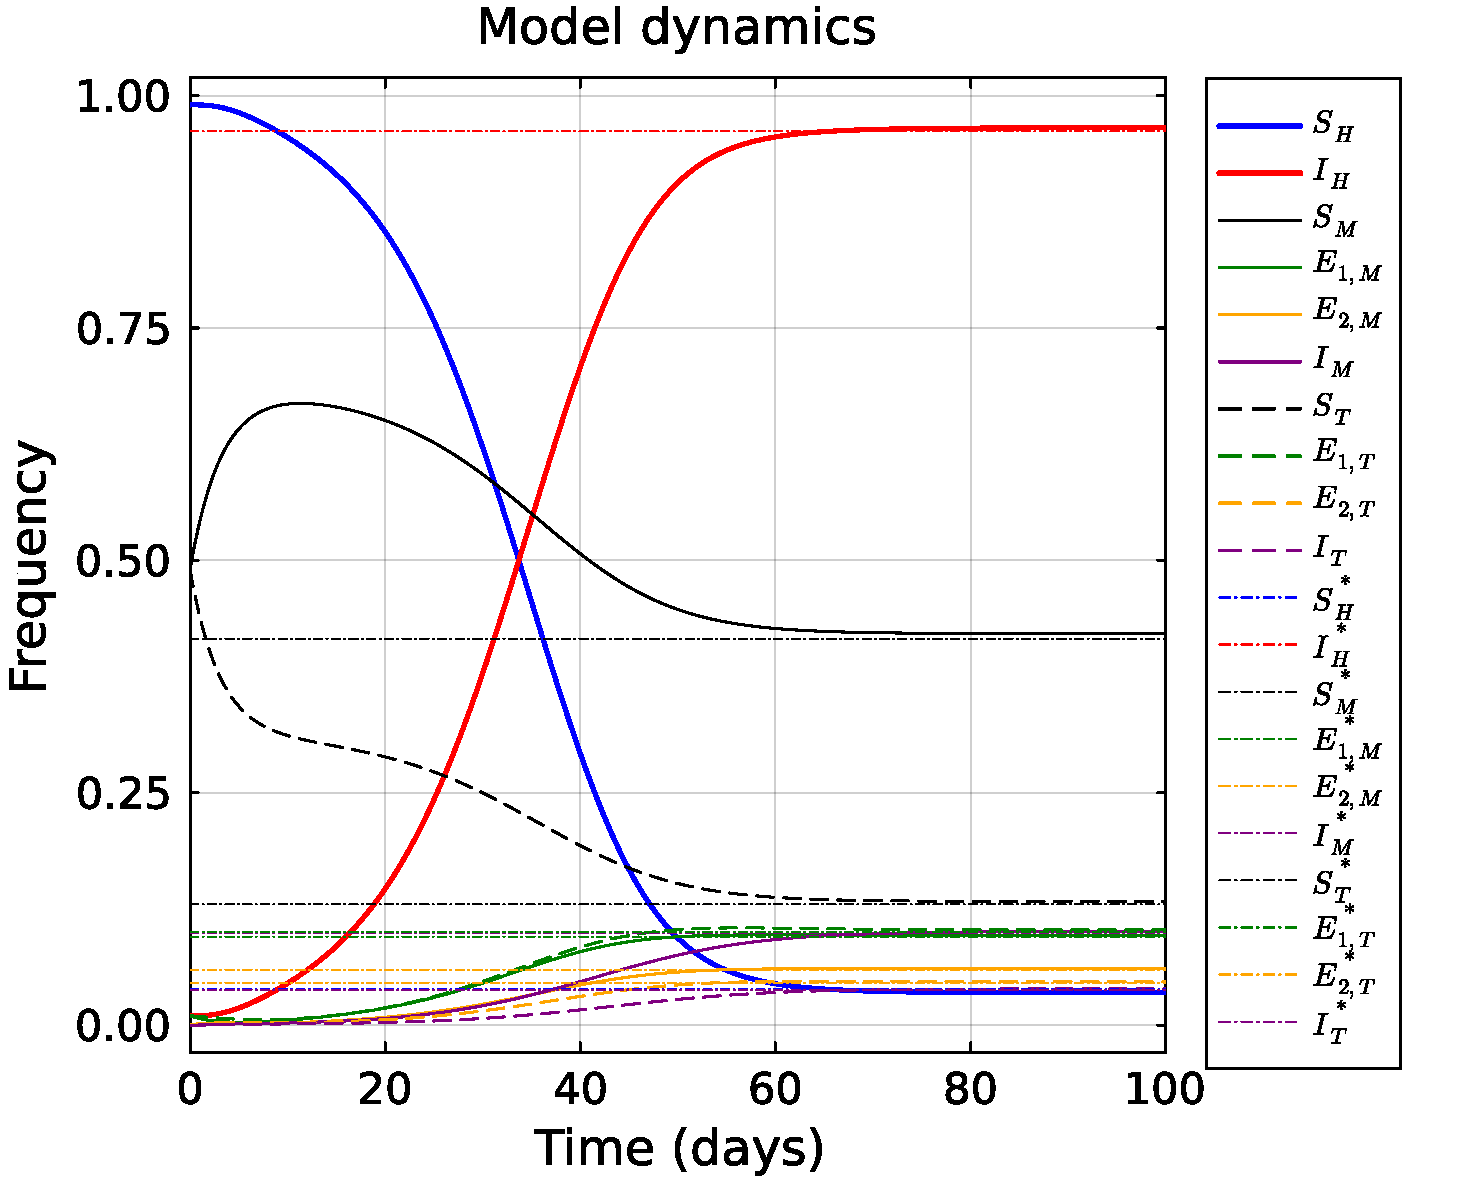
\includegraphics[width=0.8\textwidth]{../../fig/model_dynamics.pdf}
  \caption{Dynamics of the Ross-Macdonald malaria model with mosquito latency and treatment.}
\end{figure}

Now we explore the effects of varying the treatment rate $t$, the treatment waning rate $h$, and the latency progression rates. The following figures illustrate how these parameters influence the disease dynamics and equilibria.

\begin{figure}[H]
  \centering
  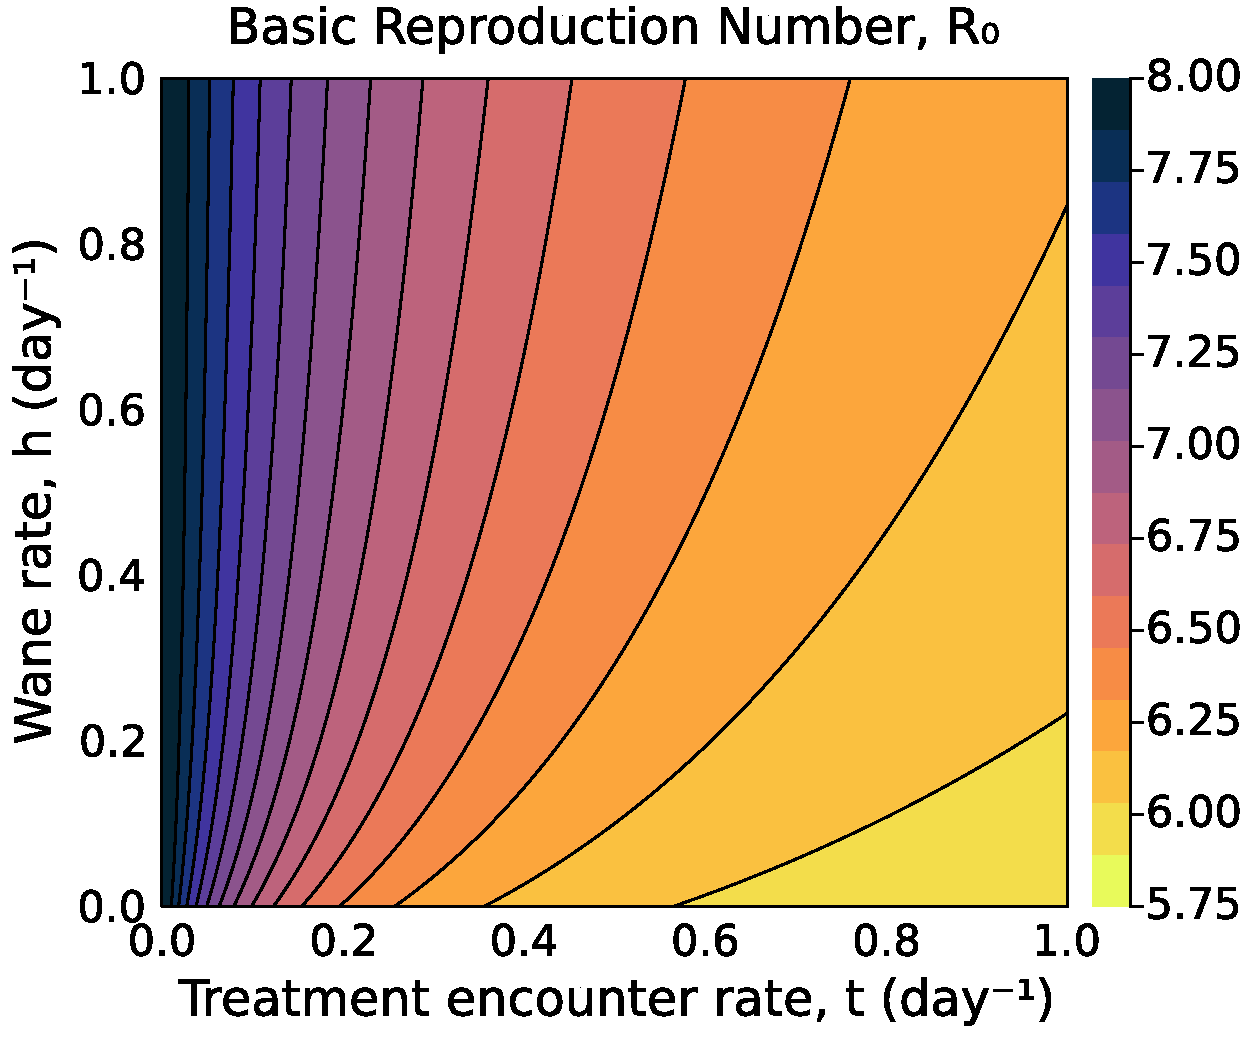
\includegraphics[width=0.4\textwidth]{../../fig/brn_txh_heatmap.pdf}
  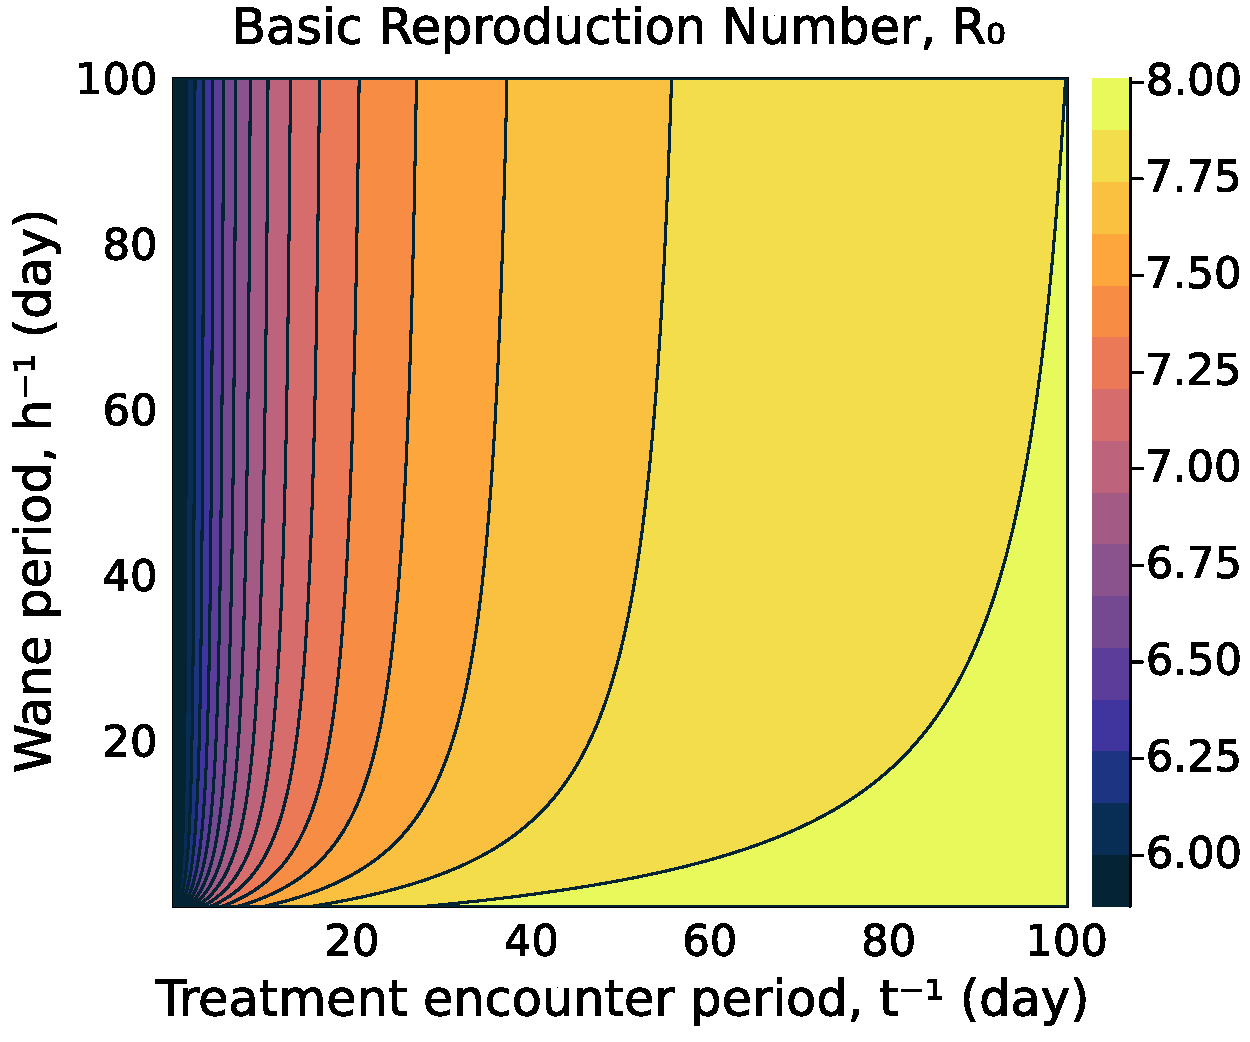
\includegraphics[width=0.4\textwidth]{../../fig/brn_txh_heatmap_rev.pdf}
  \caption{Heatmaps of the basic reproduction number $R_0$ as a function of treatment rate $t$ and treatment waning rate $h$ or treatment encounter period $t$ and treatment waning period $h$.}
\end{figure}

\begin{figure}[H]
  \centering
  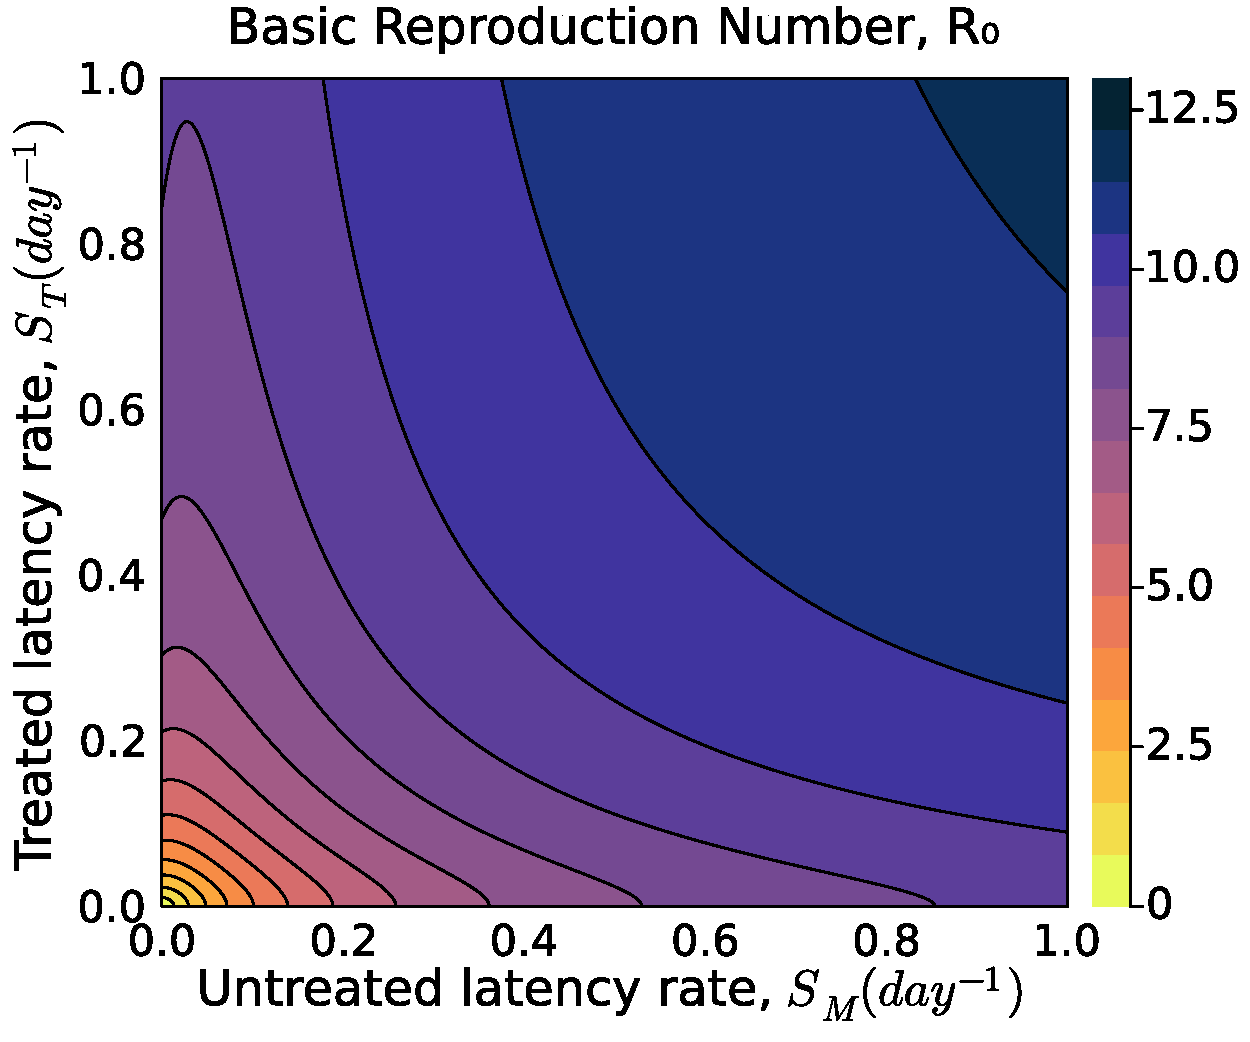
\includegraphics[width=0.4\textwidth]{../../fig/brn_smxst_heatmap.pdf}
  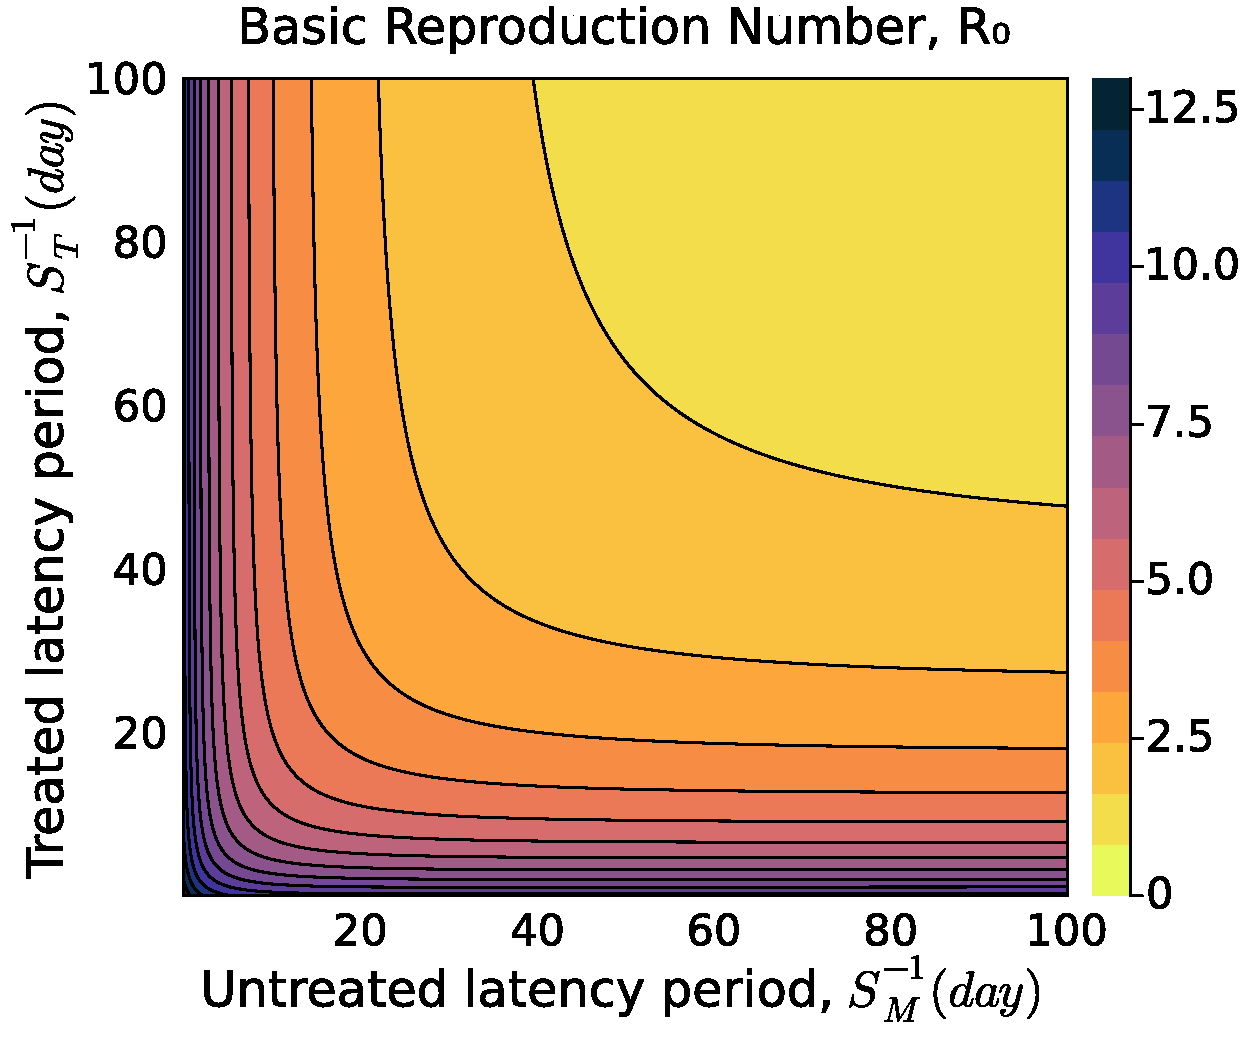
\includegraphics[width=0.4\textwidth]{../../fig/brn_smxst_heatmap_rev.pdf}
  \caption{Heatmaps of the basic reproduction number $R_0$ as a function of untreated mosquito latency progression rate $s_M$ and treated mosquito latency progression rate $s_T$ or untreated mosquito latency period $L_{NM}$ and treated mosquito latency period $L_{NT}$.}
\end{figure}

\begin{figure}[H]
  \centering
  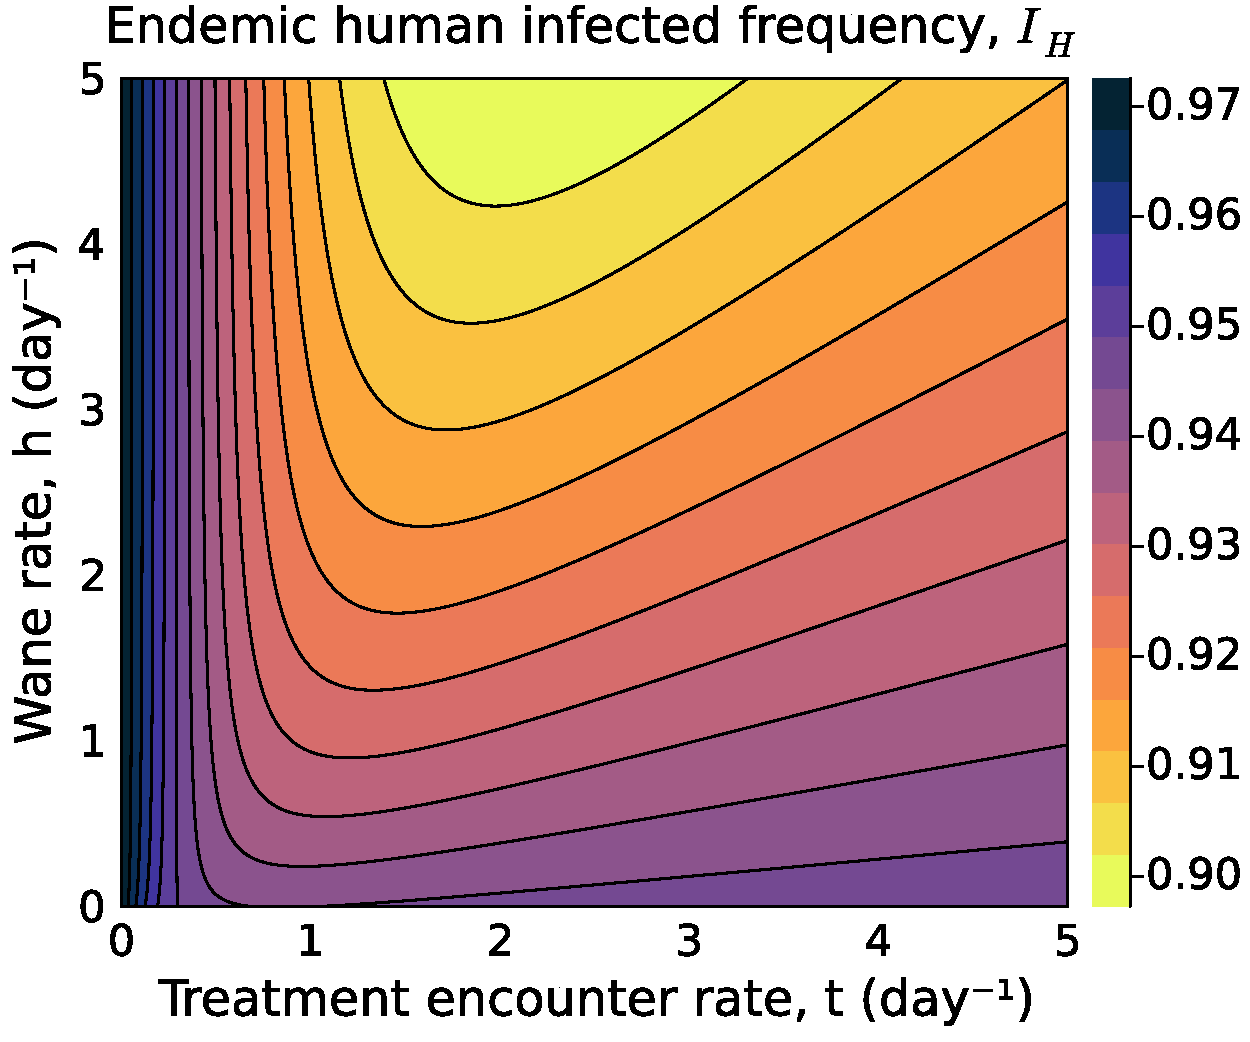
\includegraphics[width=0.4\textwidth]{../../fig/Ih_txh.pdf}
  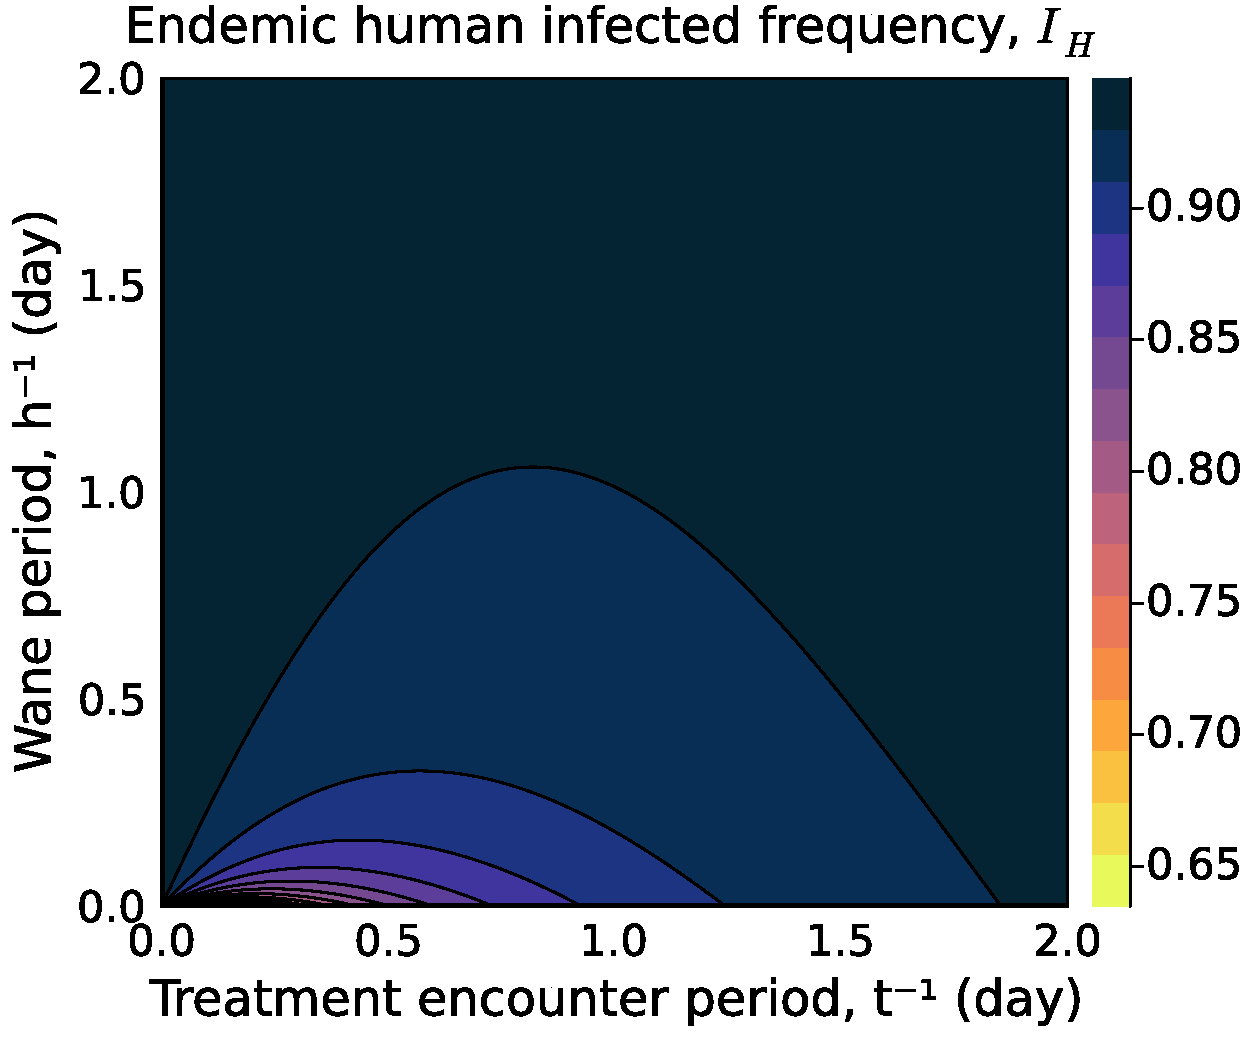
\includegraphics[width=0.4\textwidth]{../../fig/Ih_txh_rev.pdf}
  \caption{Heatmaps of the human infected proportion $I_H^*$ at equilibrium (prevalence) as a function of treatment rate $t$ and treatment waning rate $h$ or treatment encounter period $t$ and treatment waning period $h$.}
\end{figure}

\begin{figure}[H]
  \centering
  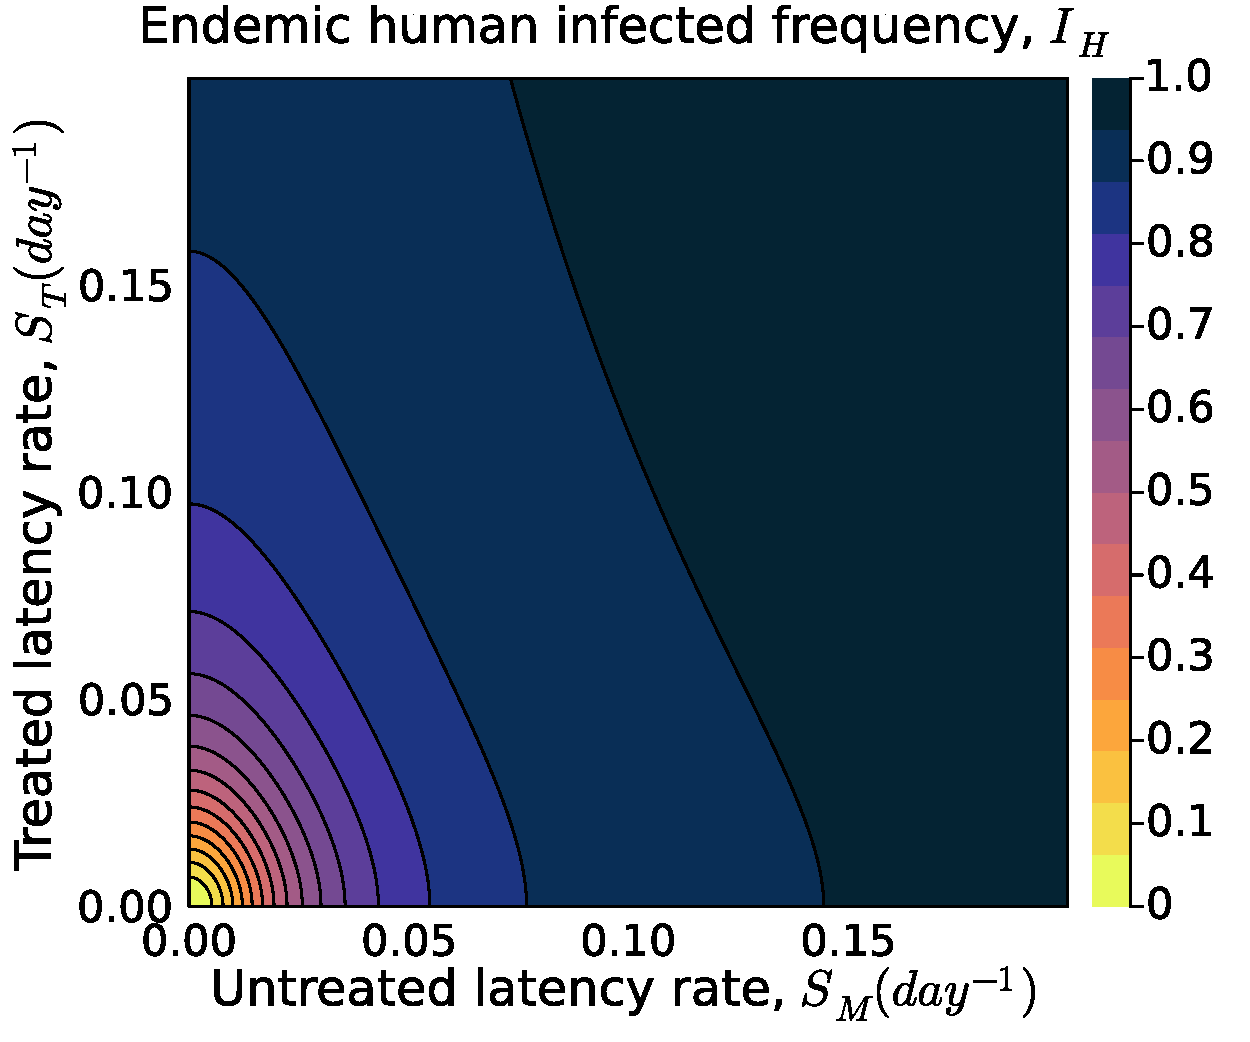
\includegraphics[width=0.4\textwidth]{../../fig/Ih_STxSM.pdf}
  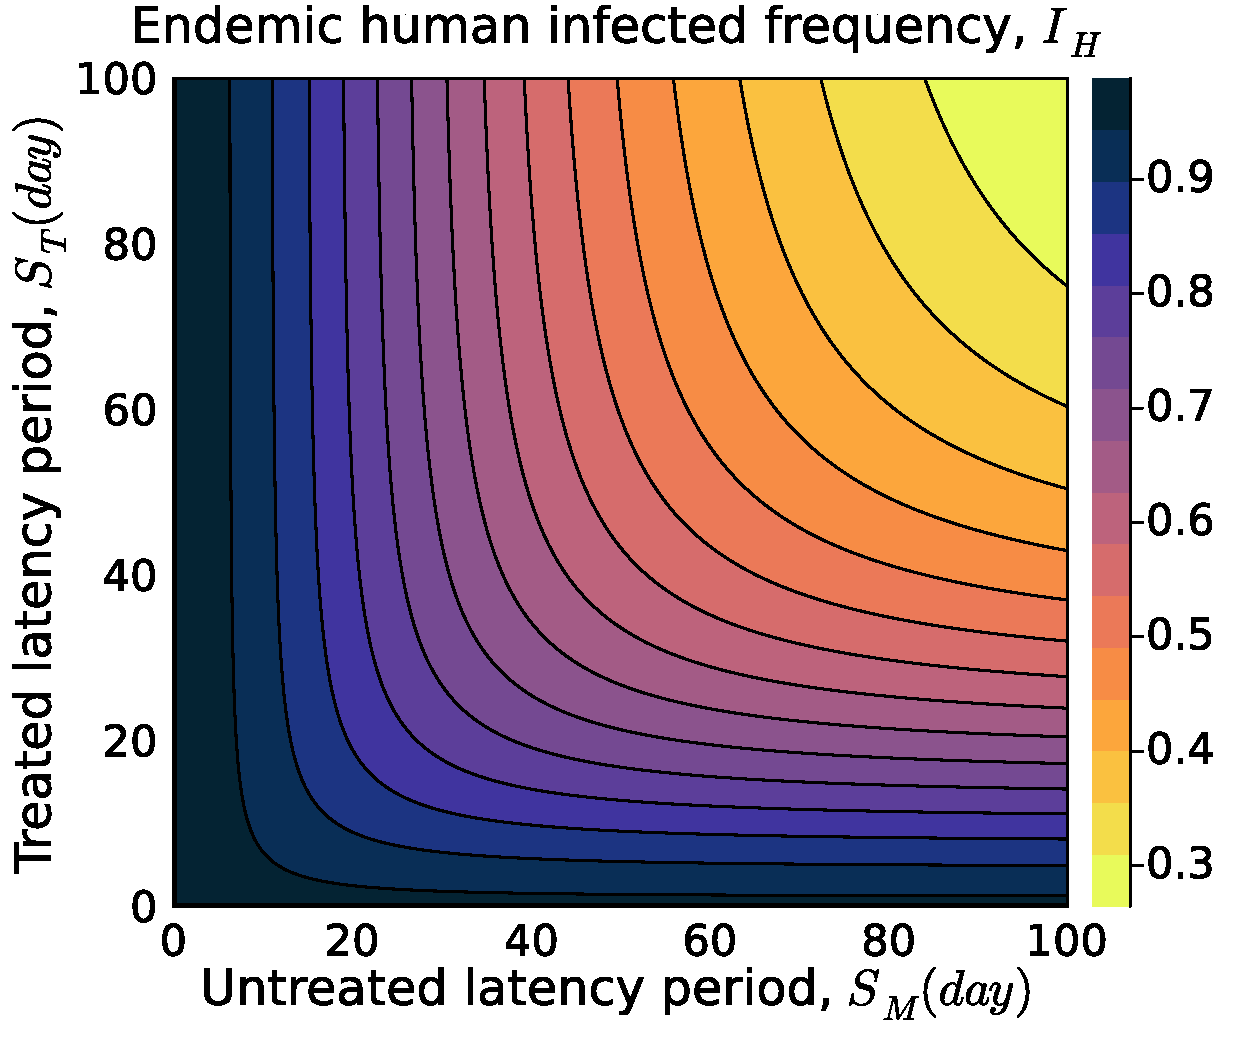
\includegraphics[width=0.4\textwidth]{../../fig/Ih_STxSM_rev.pdf}
  \caption{Heatmaps of the human infected proportion $I_H^*$ at equilibrium (prevalence) as a function of untreated mosquito latency progression rate $s_M$ and treated mosquito latency progression rate $s_T$ or untreated mosquito latency period $L_{NM}$ and treated mosquito latency period $L_{NT}$.}
\end{figure}

Now we employ the erlang distribution to generalize the mosquito latency with arbitrary number of stages. The following figures illustrate the effects of varying the number of latent stages for untreated and treated mosquitoes on the basic reproduction number $R_0$ and the human infected proportion $I_H^*$ at equilibrium.

\begin{figure}[H]
  \centering
  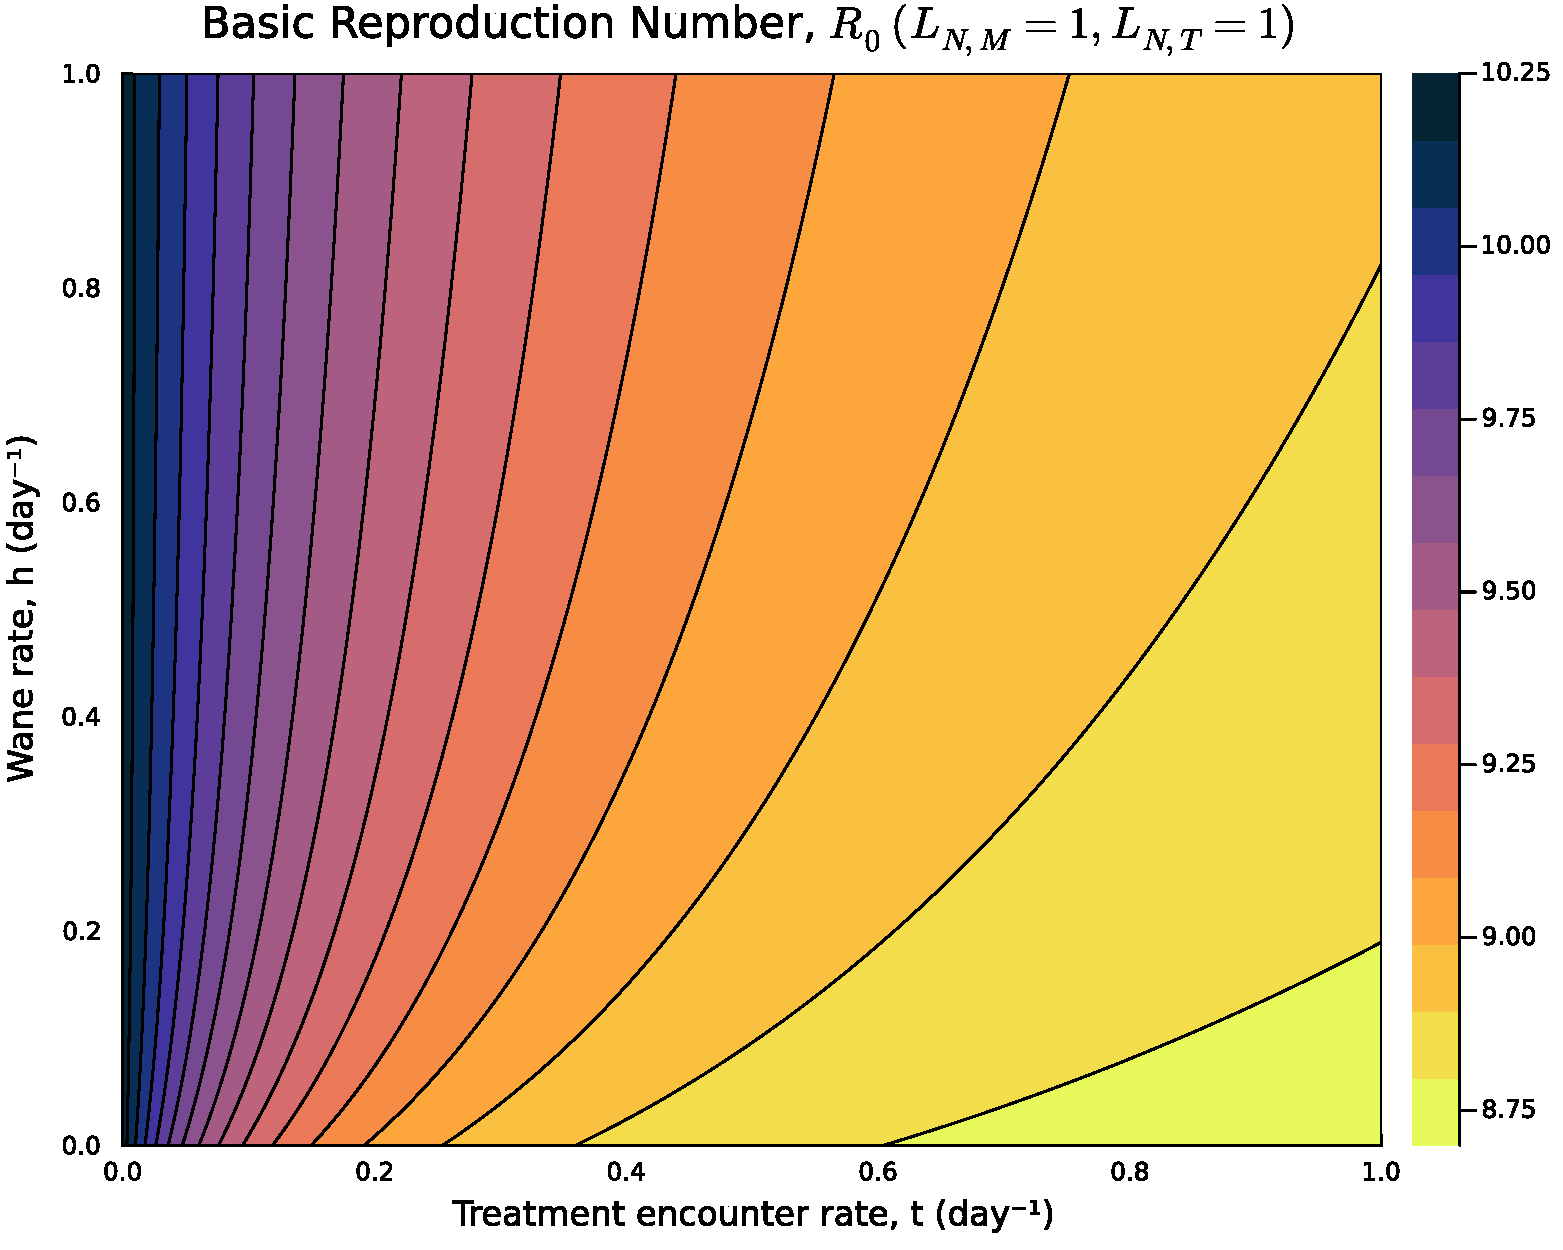
\includegraphics[width=0.4\textwidth]{../../fig/R0_rates_txh_1x1_uncal.pdf}
  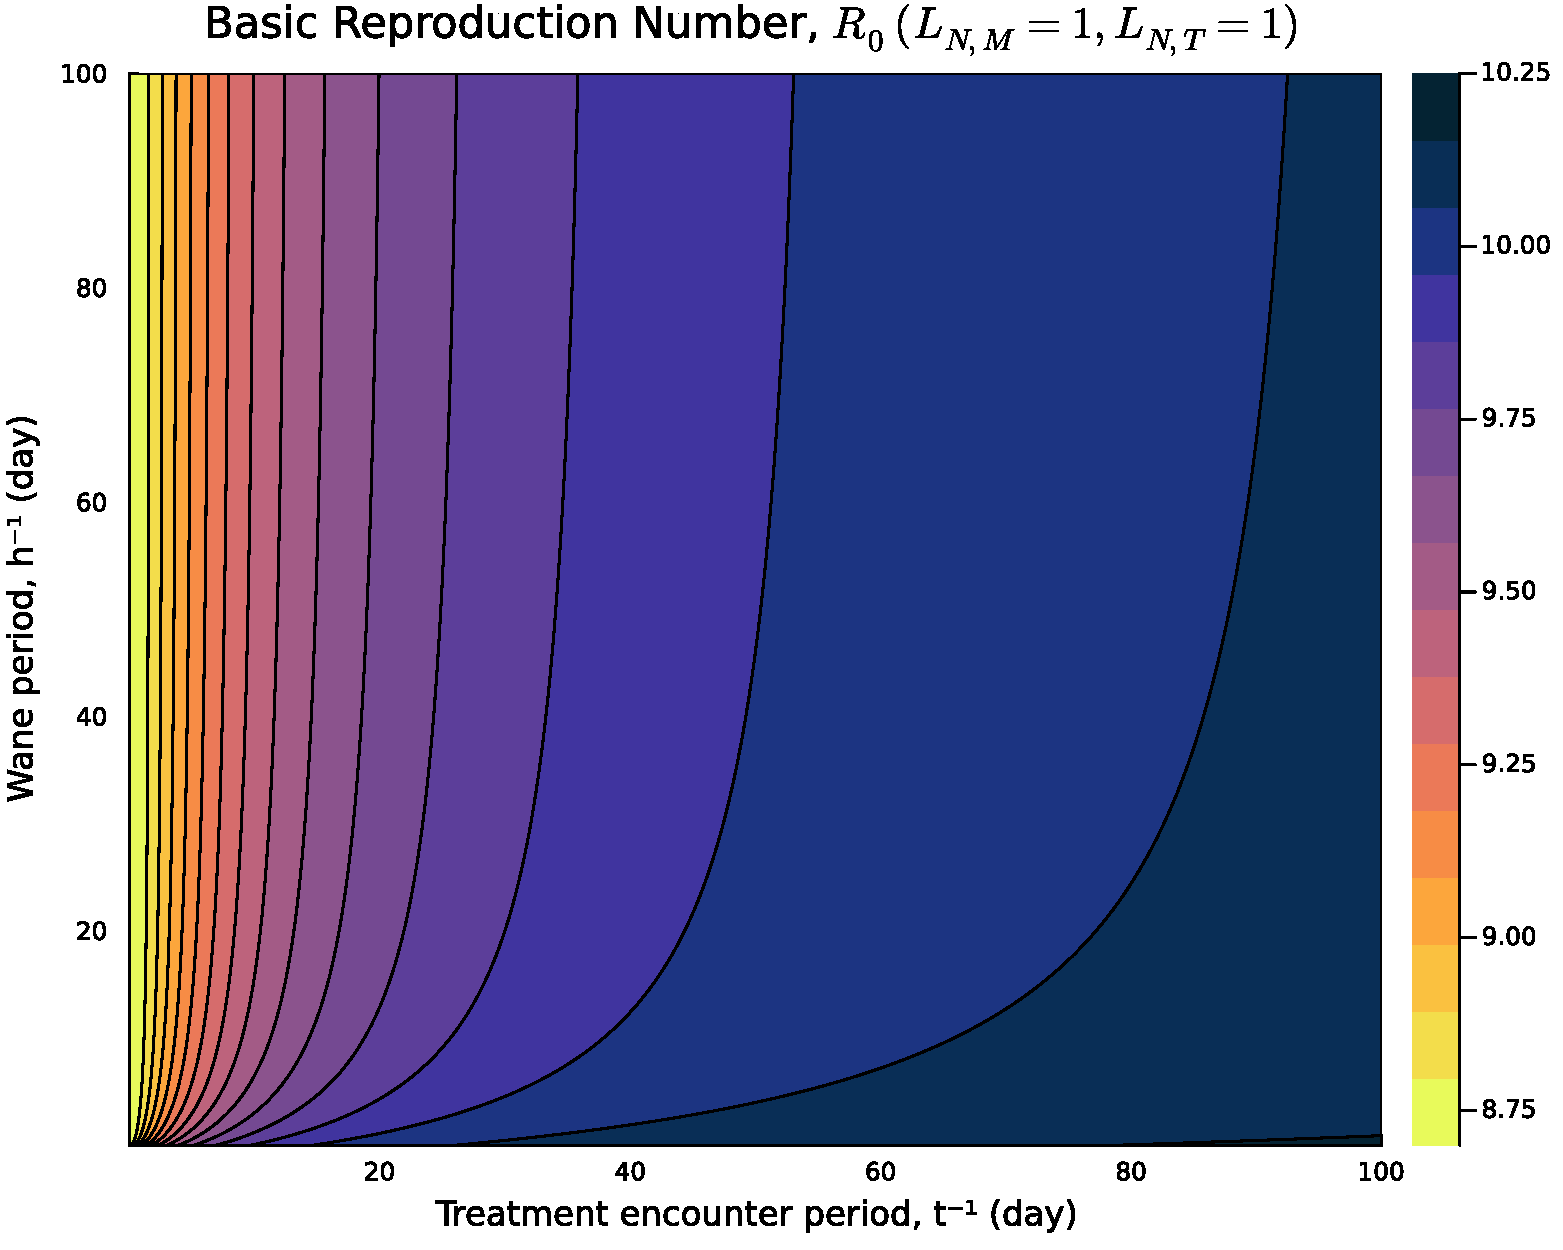
\includegraphics[width=0.4\textwidth]{../../fig/R0_periods_txh_1x1_uncal.pdf}\\
  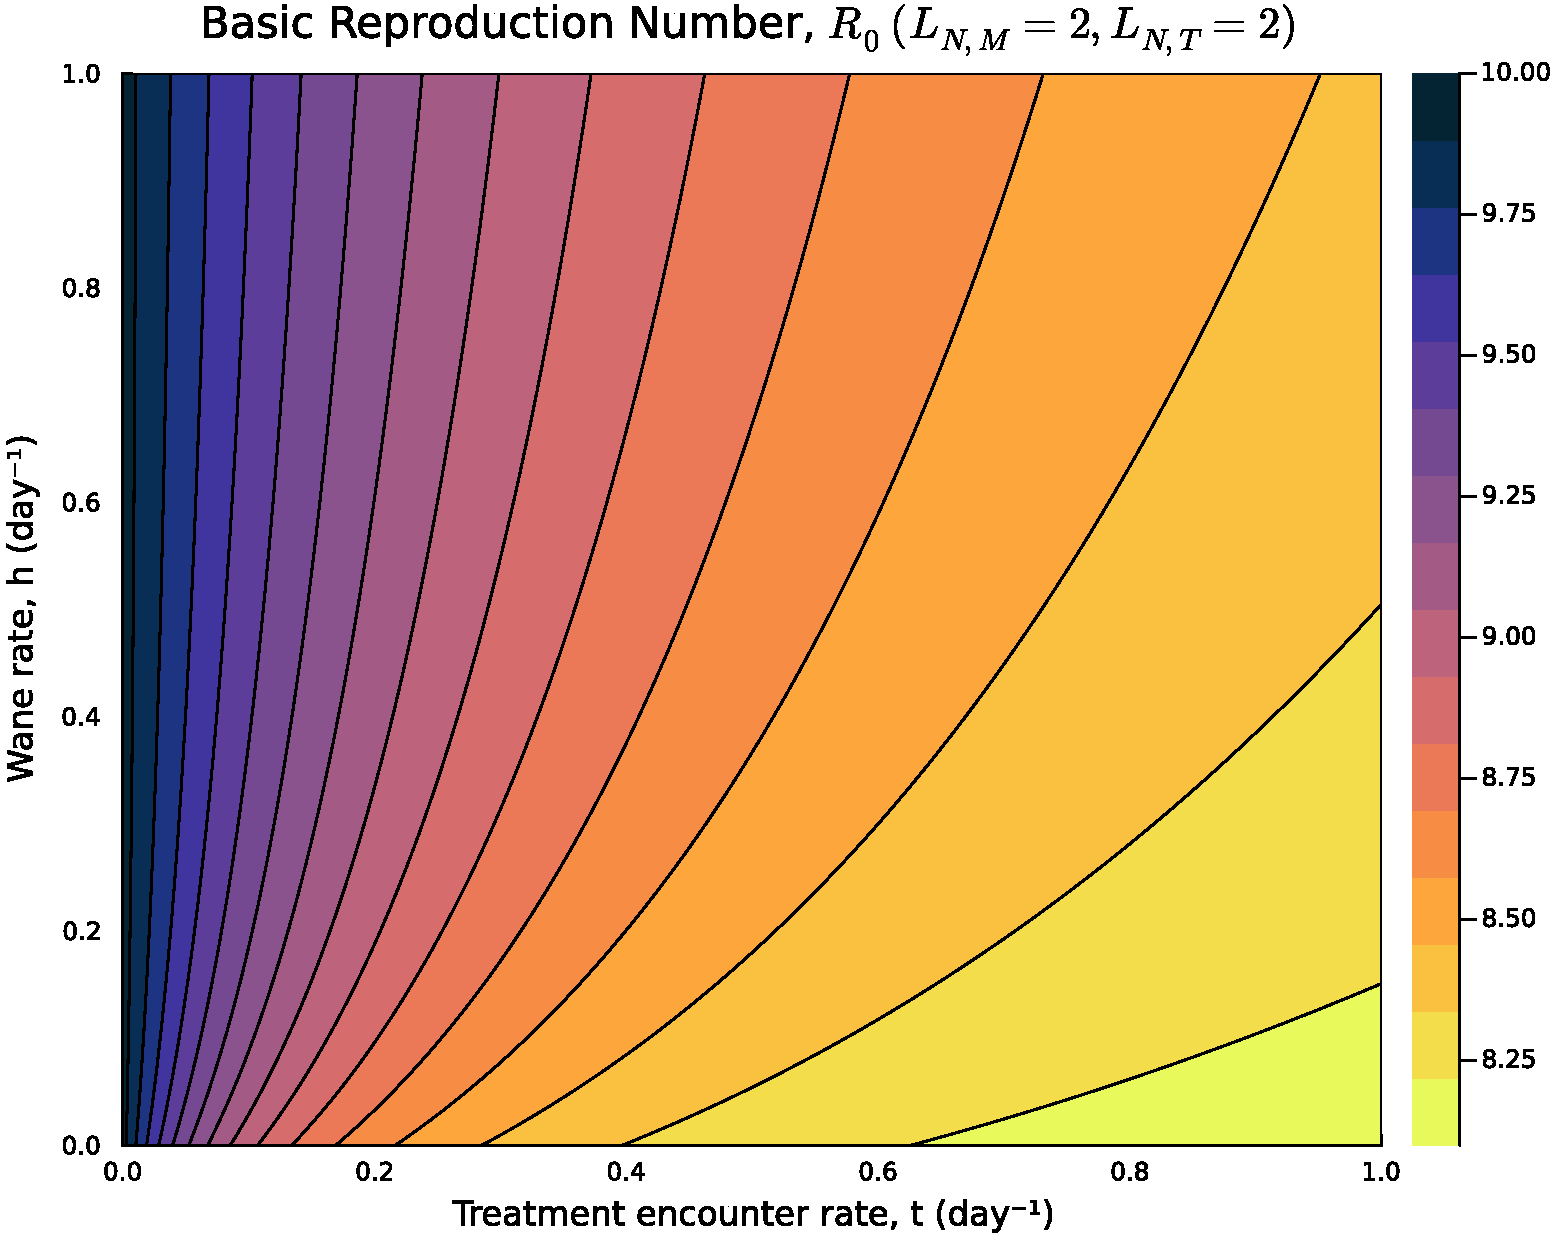
\includegraphics[width=0.4\textwidth]{../../fig/R0_rates_txh_2x2_uncal.pdf}
  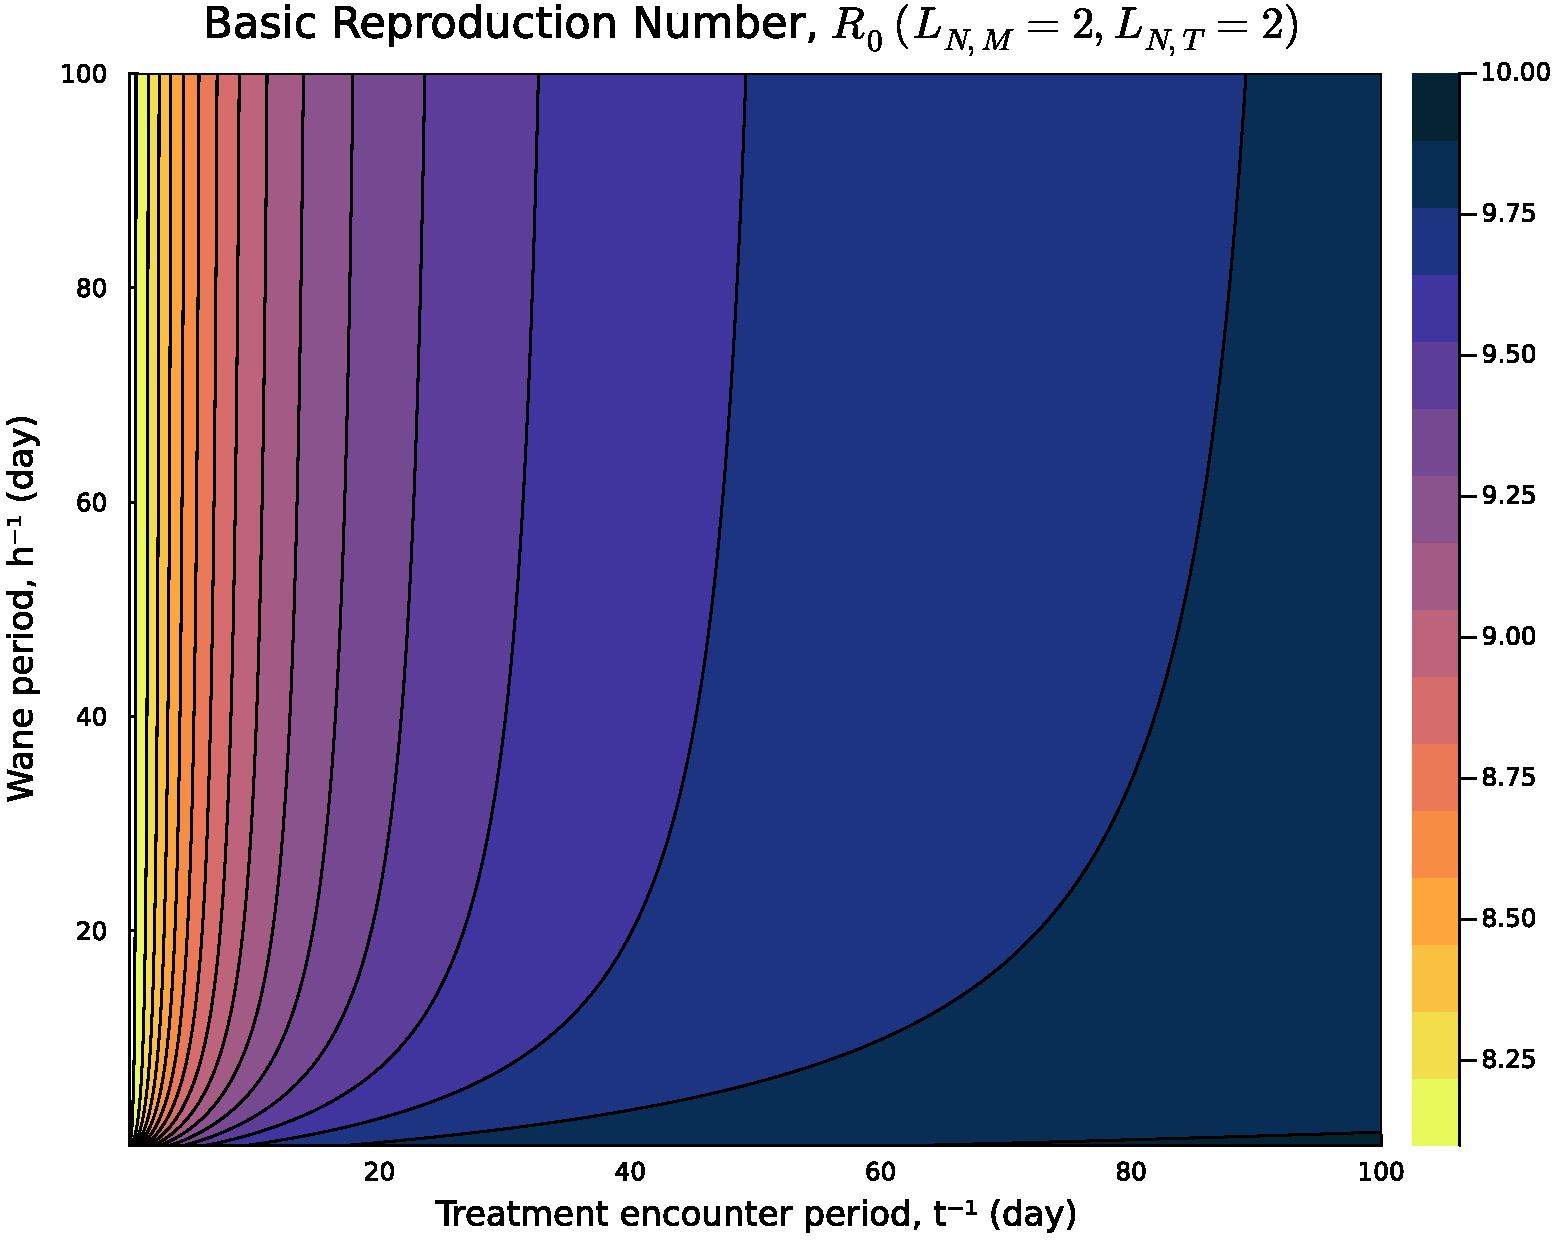
\includegraphics[width=0.4\textwidth]{../../fig/R0_periods_txh_2x2_uncal.pdf}\\
  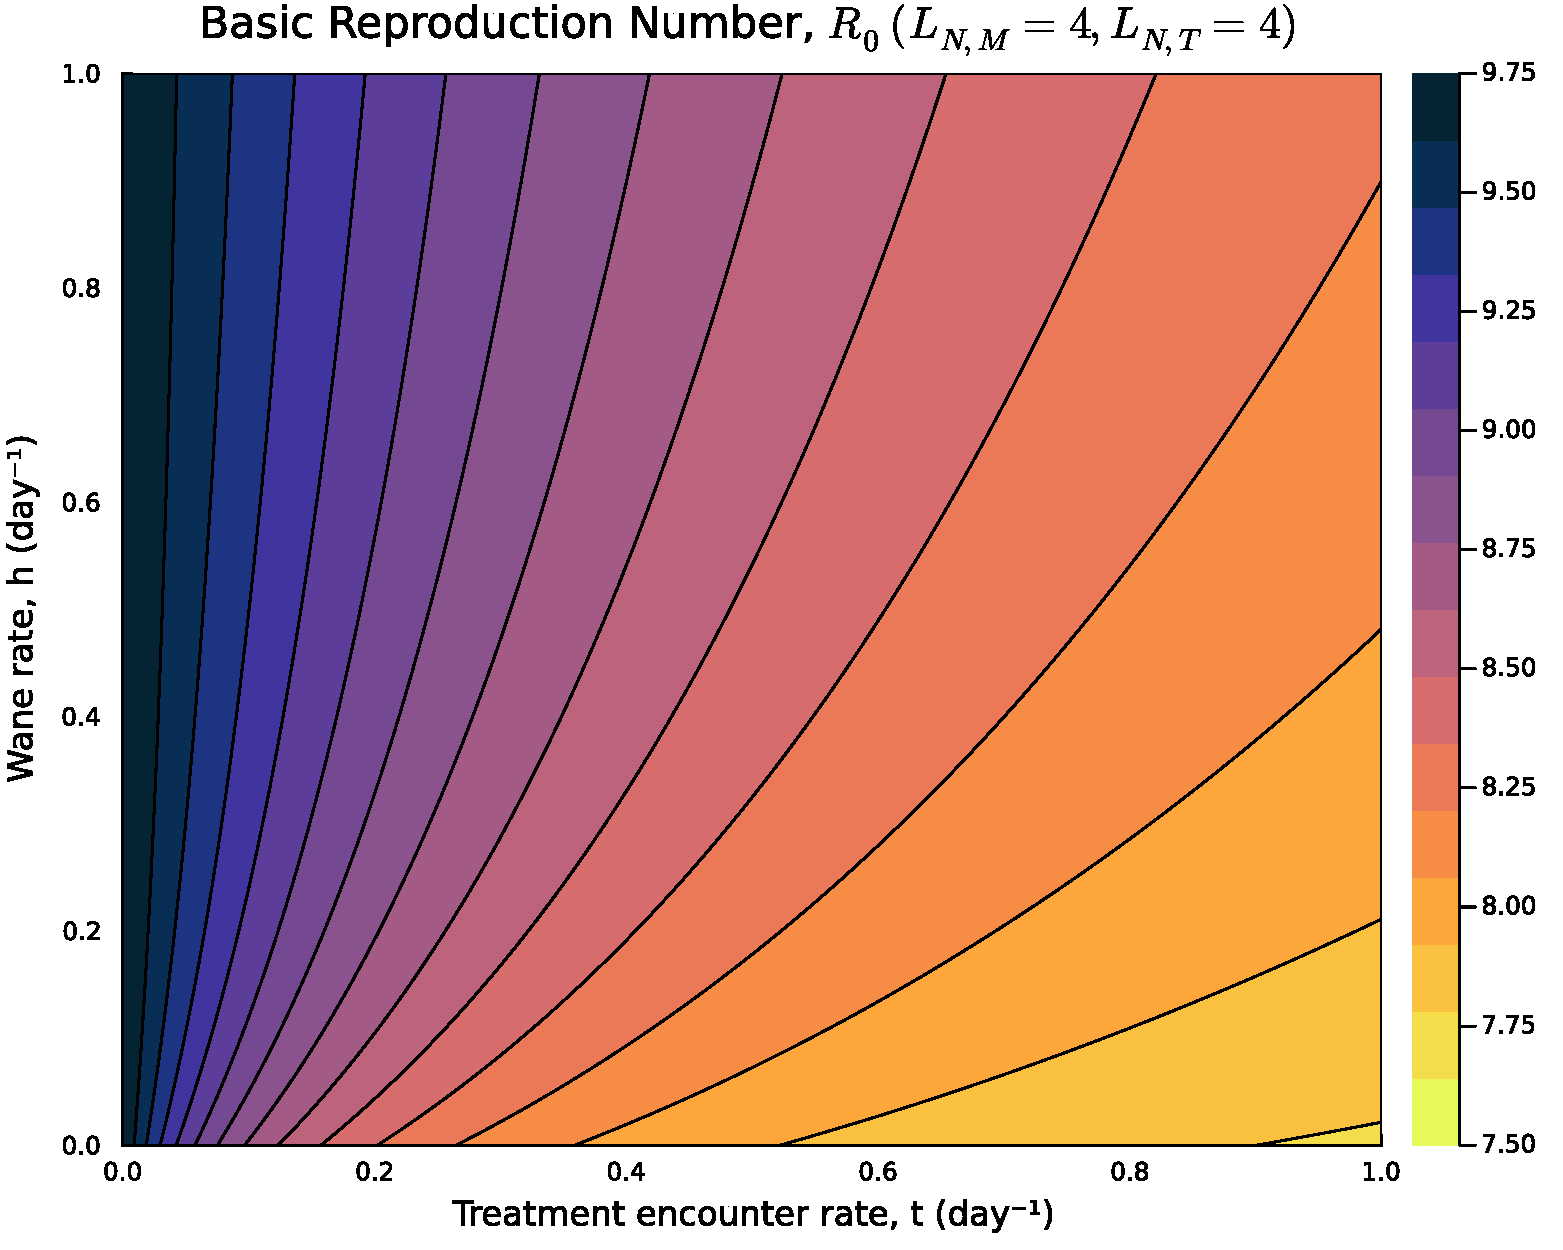
\includegraphics[width=0.4\textwidth]{../../fig/R0_rates_txh_4x4_uncal.pdf}
  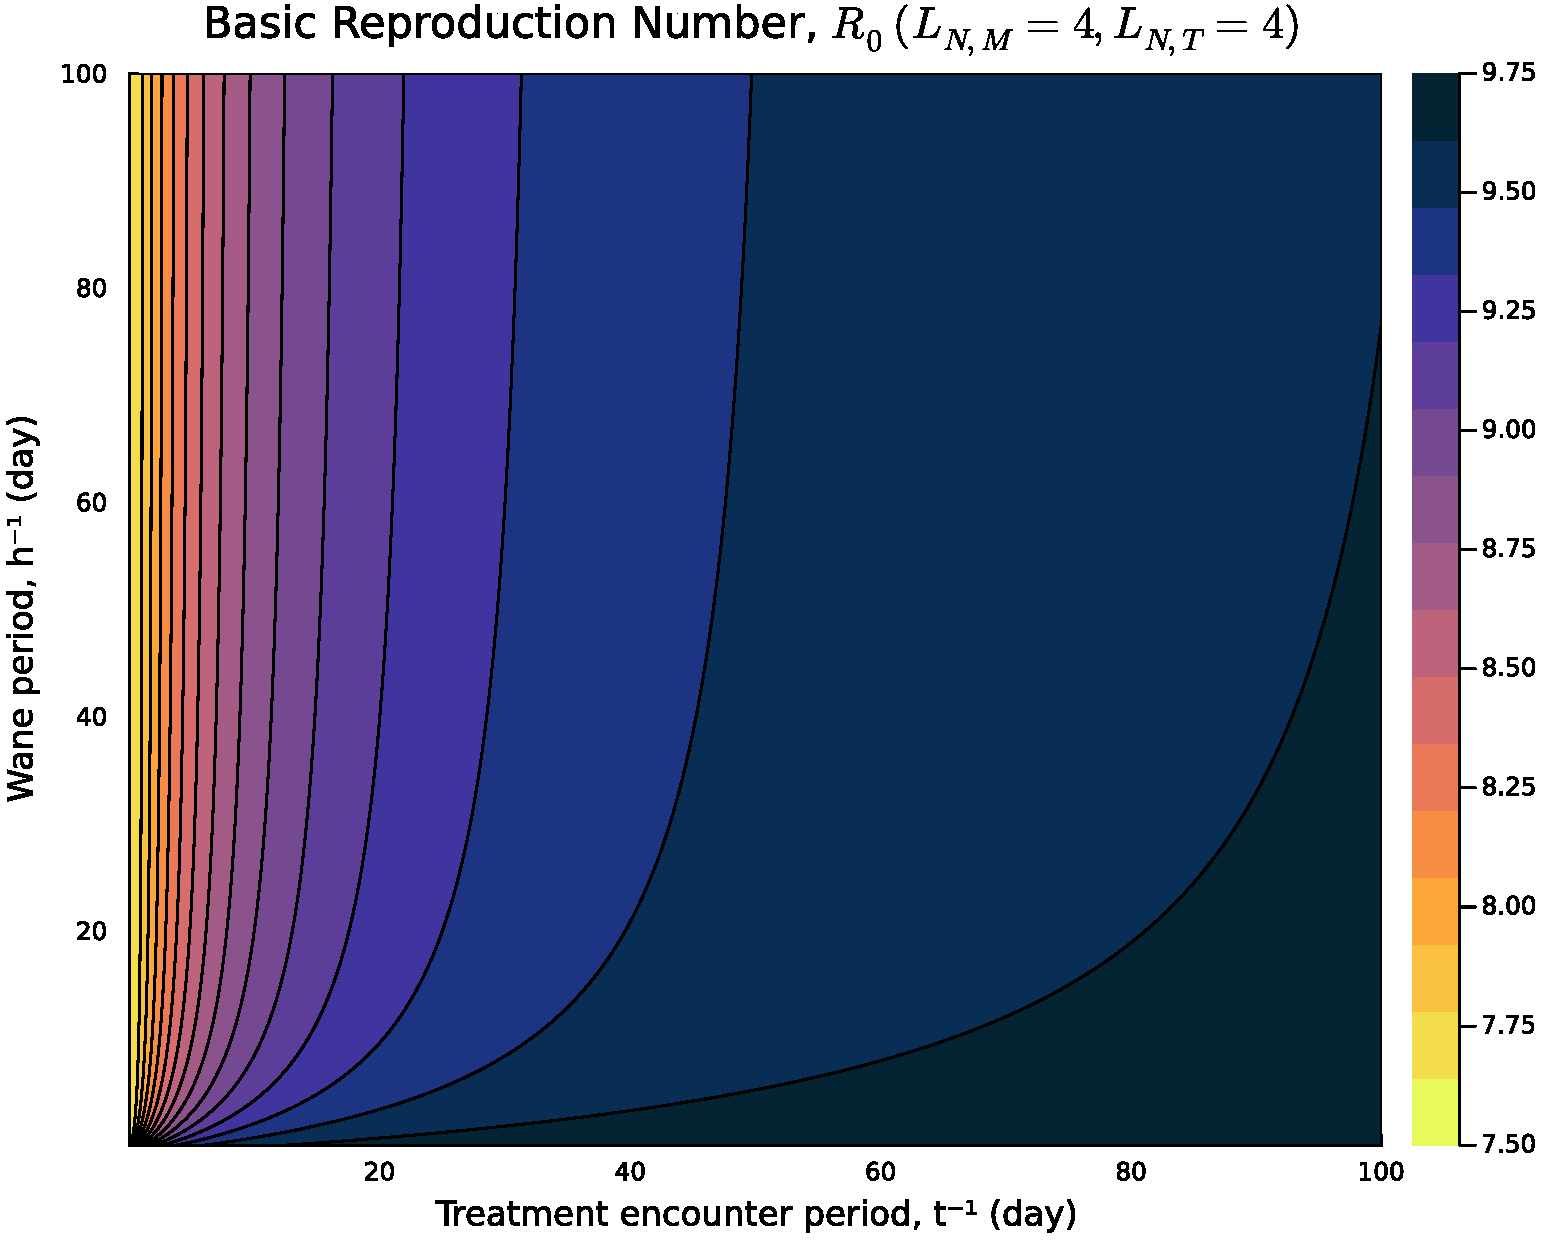
\includegraphics[width=0.4\textwidth]{../../fig/R0_periods_txh_4x4_uncal.pdf}
  \caption{Heatmaps of the basic reproduction number $R_0$ as a function of treatment rate $t$ and treatment waning rate $h$ or treatment encounter period $t$ and treatment waning period $h$ for the generalized model with erlang-distributed mosquito latency with 1, 2, and 4 latency stages for both untreated and treated mosquitoes.}
\end{figure}

\begin{figure}[H]
  \centering
  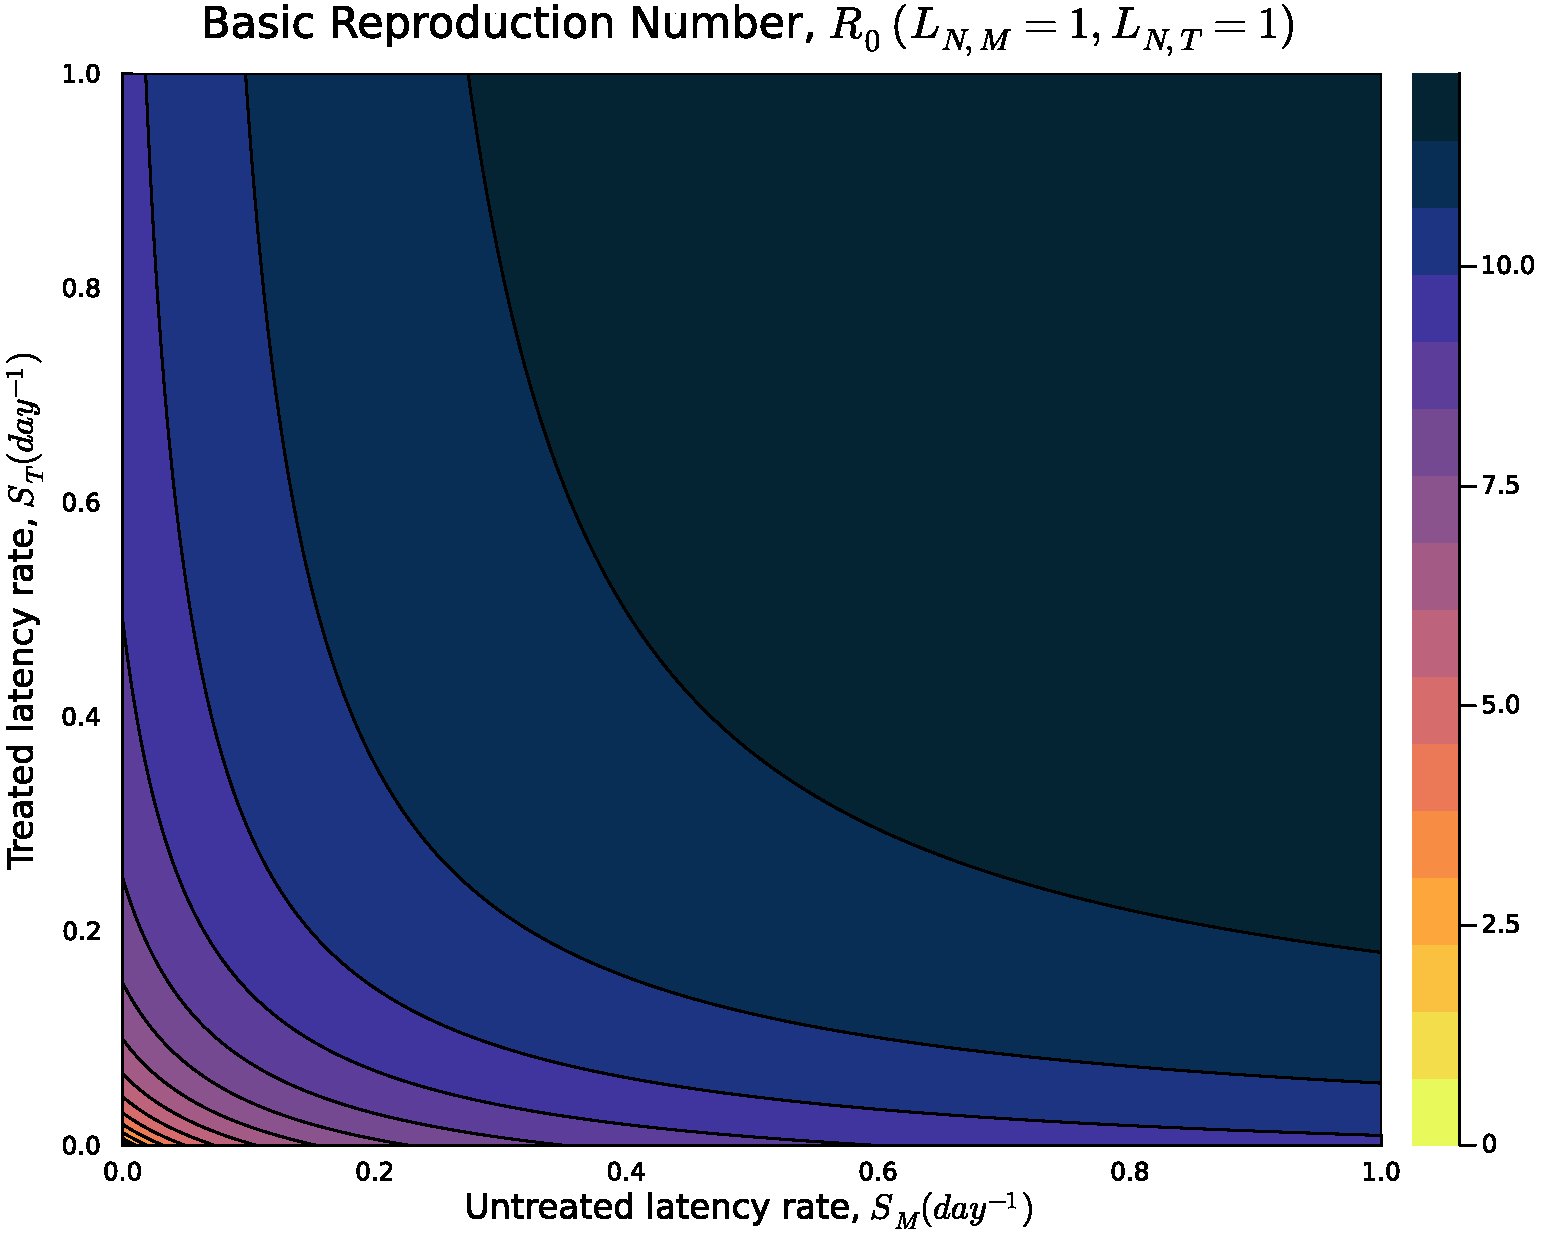
\includegraphics[width=0.4\textwidth]{../../fig/R0_rates_SMxST_1x1_uncal.pdf}
  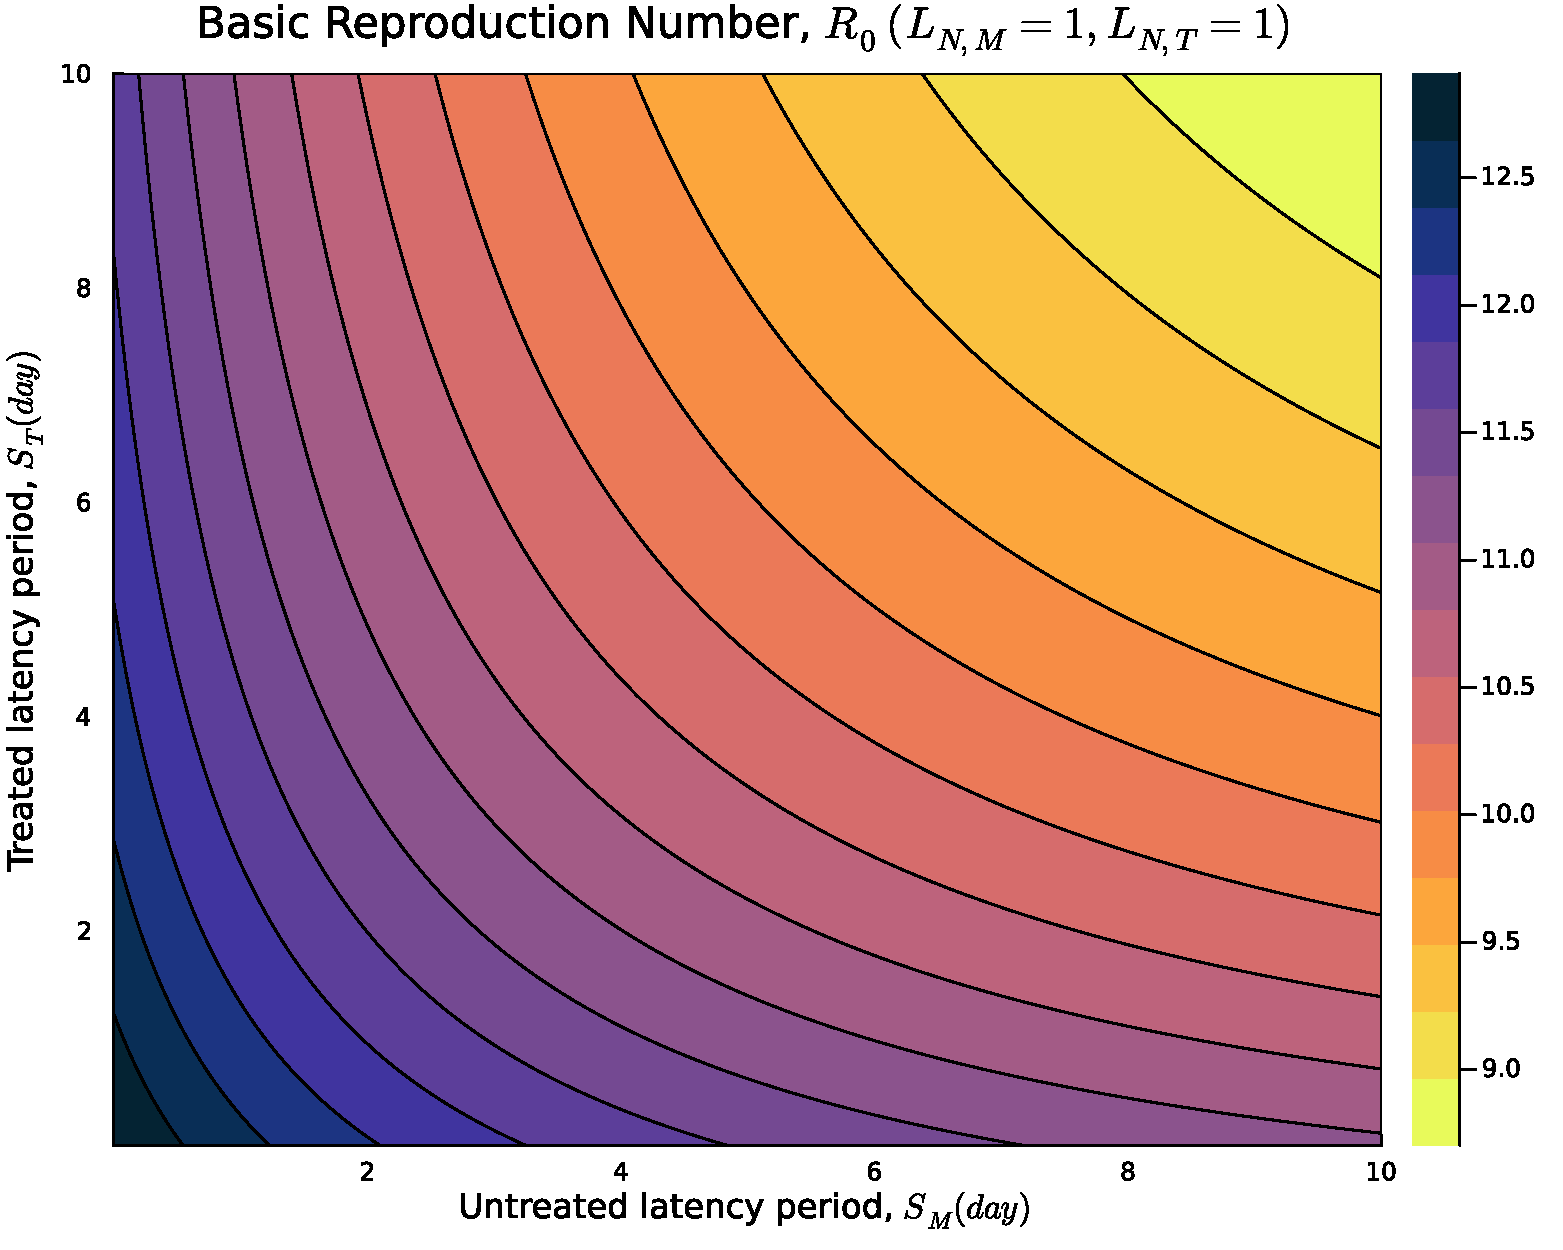
\includegraphics[width=0.4\textwidth]{../../fig/R0_periods_SMxST_1x1_uncal.pdf}\\
  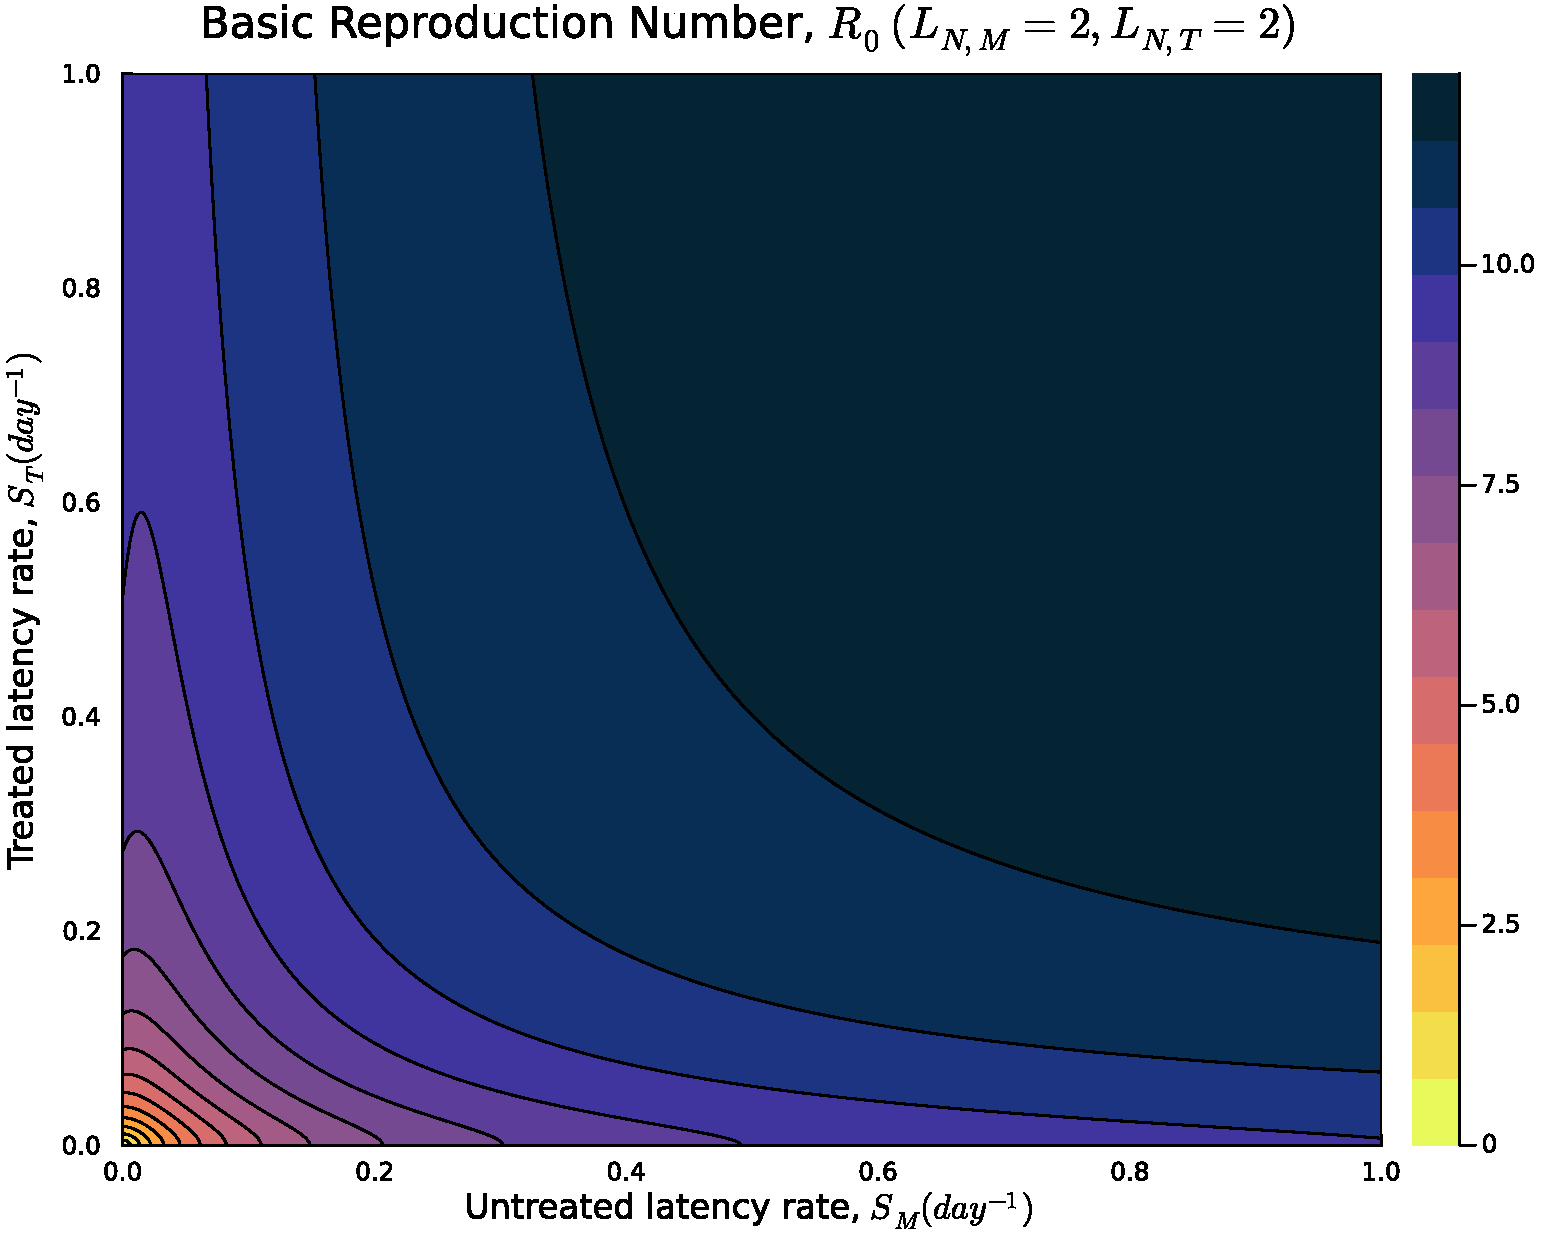
\includegraphics[width=0.4\textwidth]{../../fig/R0_rates_SMxST_2x2_uncal.pdf}
  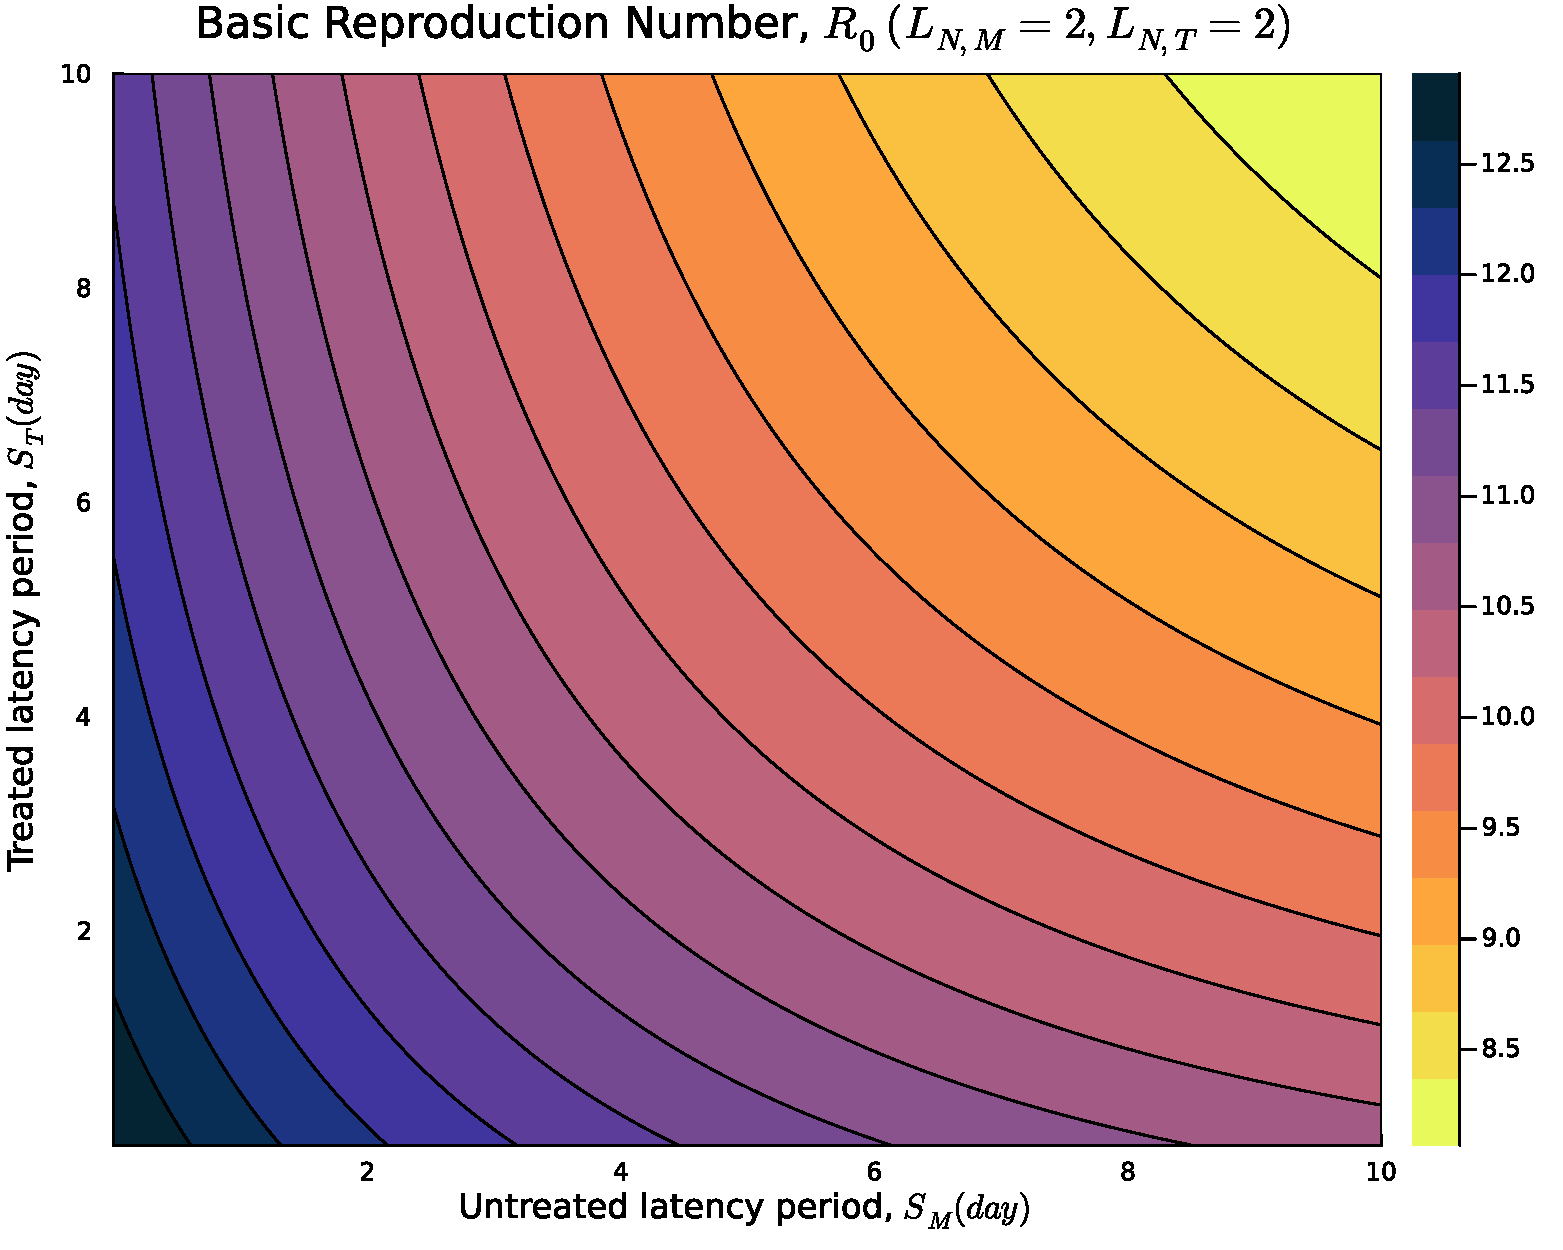
\includegraphics[width=0.4\textwidth]{../../fig/R0_periods_SMxST_2x2_uncal.pdf}\\
  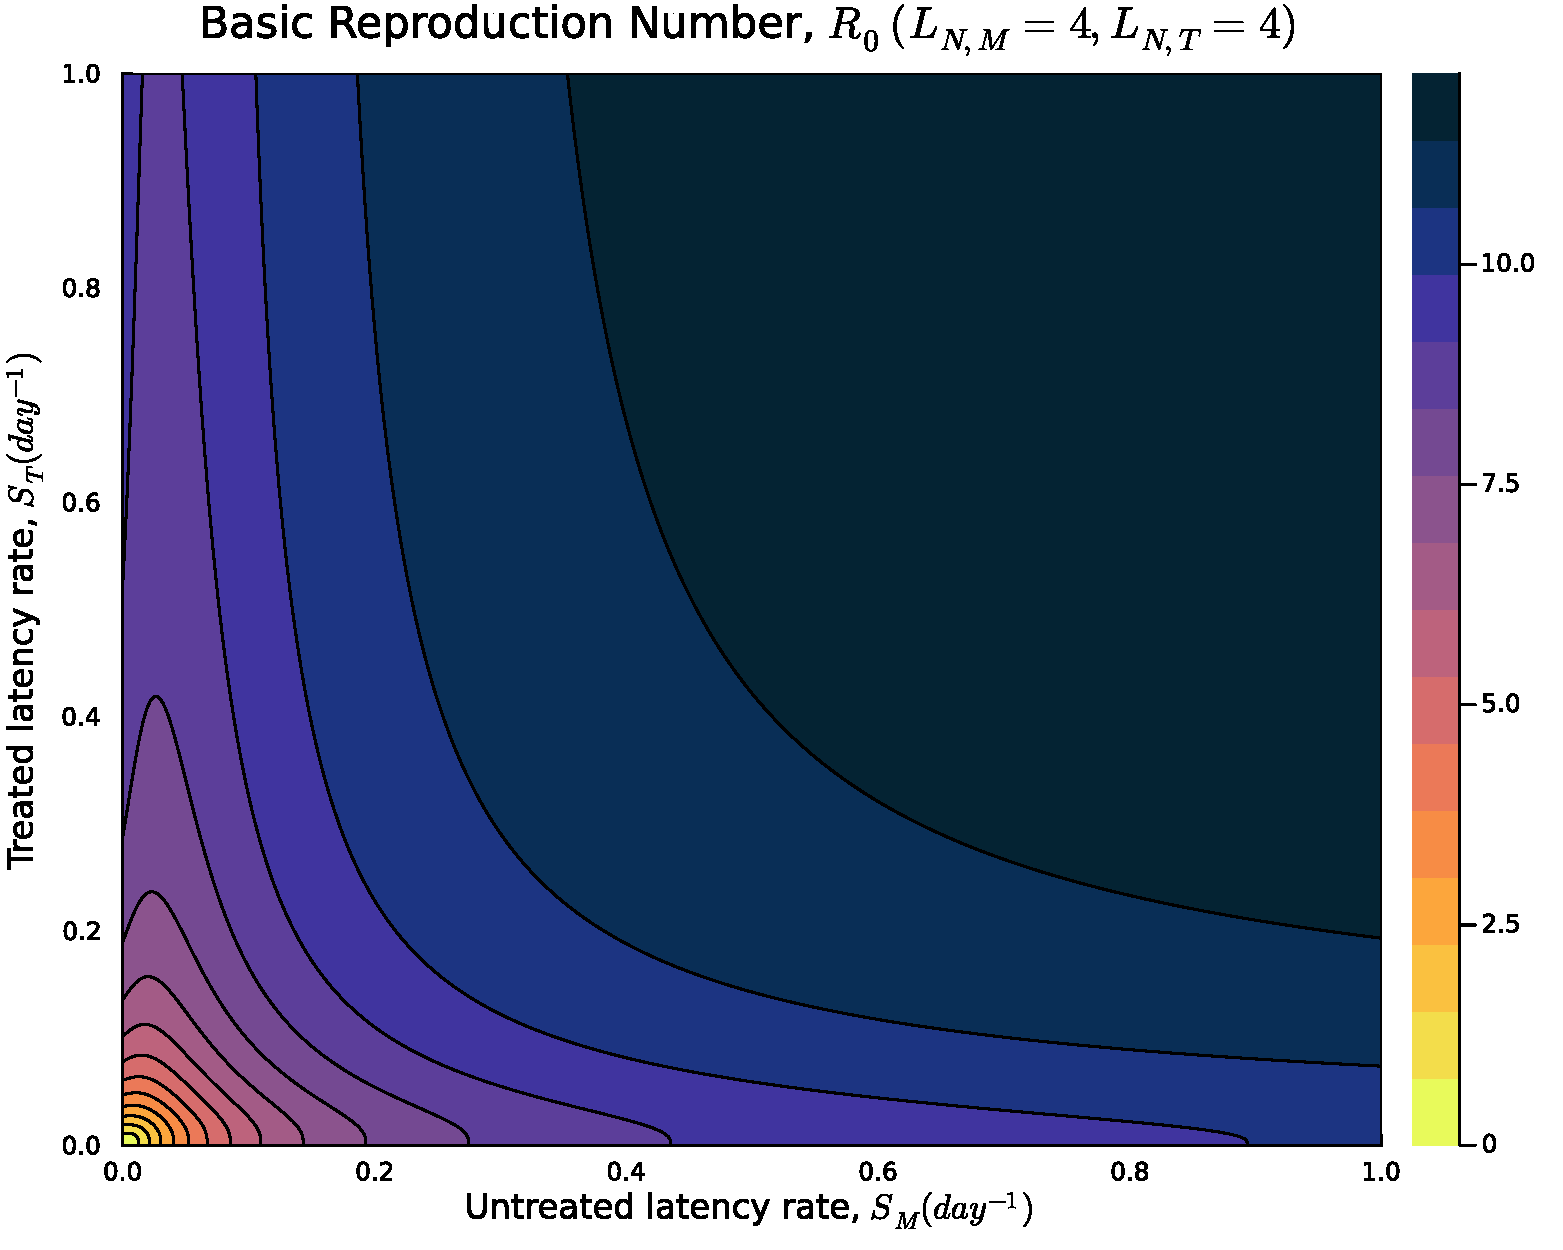
\includegraphics[width=0.4\textwidth]{../../fig/R0_rates_SMxST_4x4_uncal.pdf}
  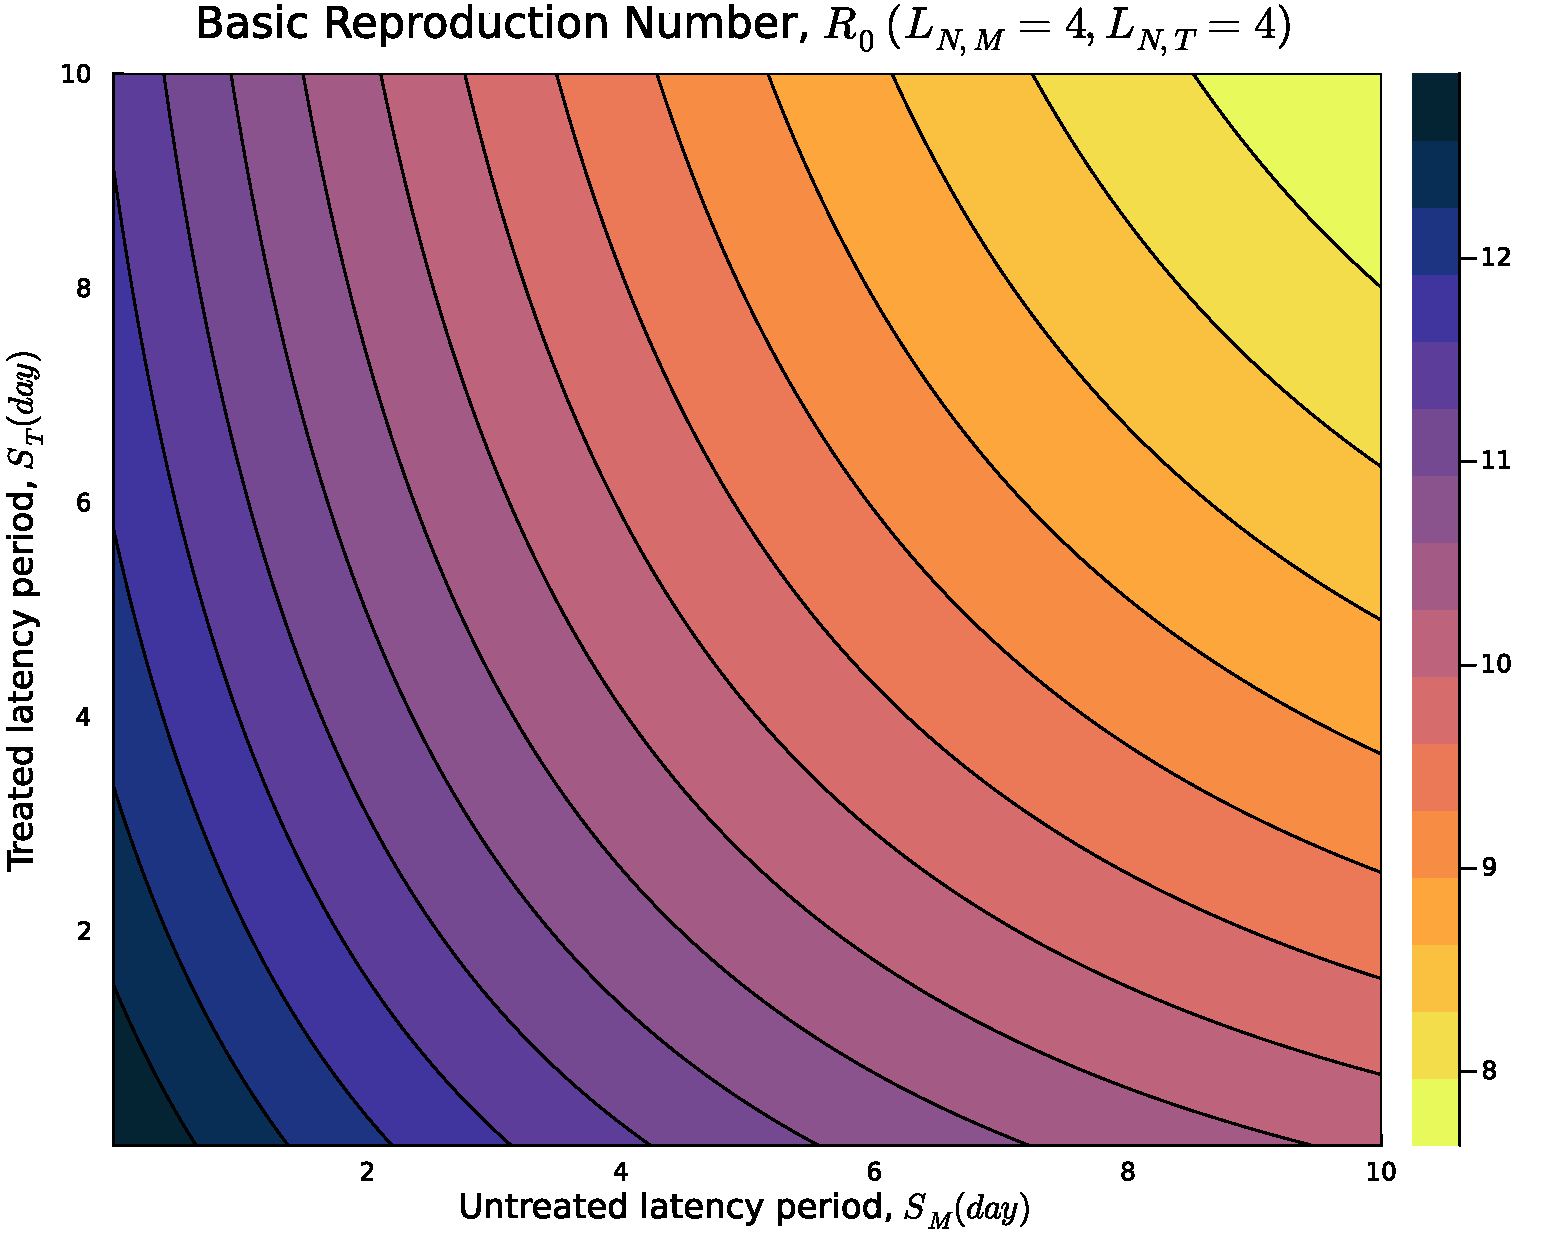
\includegraphics[width=0.4\textwidth]{../../fig/R0_periods_SMxST_4x4_uncal.pdf}
  \caption{Heatmaps of the basic reproduction number $R_0$ as a function of untreated mosquito latency progression rate $s_M$ and treated mosquito latency progression rate $s_T$ or untreated mosquito latency period $L_{NM}$ and treated mosquito latency period $L_{NT}$ for the generalized model with erlang-distributed mosquito latency with 1, 2, and 4 latency stages for both untreated and treated mosquitoes.}
\end{figure}

\begin{figure}[H]
  \centering
  \includegraphics[width=0.4\textwidth]{../../fig/Ih_rates_txh_1x1_uncal.pdf}
  \includegraphics[width=0.4\textwidth]{../../fig/Ih_periods_txh_1x1_uncal.pdf}\\
  \includegraphics[width=0.4\textwidth]{../../fig/Ih_rates_txh_2x2_uncal.pdf}
  \includegraphics[width=0.4\textwidth]{../../fig/Ih_periods_txh_2x2_uncal.pdf}\\
  \includegraphics[width=0.4\textwidth]{../../fig/Ih_rates_txh_4x4_uncal.pdf}
  \includegraphics[width=0.4\textwidth]{../../fig/Ih_periods_txh_4x4_uncal.pdf}
  \caption{Heatmaps of the human infected proportion $I_H^*$ at equilibrium (prevalence) as a function of treatment rate $t$ and treatment waning rate $h$ or treatment encounter period $t$ and treatment waning period $h$ for the generalized model with erlang-distributed mosquito latency with 1, 2, and 4 latency stages for both untreated and treated mosquitoes.}
\end{figure}

\begin{figure}[H]
  \centering
  \includegraphics[width=0.4\textwidth]{../../fig/Ih_rates_SMxST_1x1_uncal.pdf}
  \includegraphics[width=0.4\textwidth]{../../fig/Ih_periods_SMxST_1x1_uncal.pdf}\\
  \includegraphics[width=0.4\textwidth]{../../fig/Ih_rates_SMxST_2x2_uncal.pdf}
  \includegraphics[width=0.4\textwidth]{../../fig/Ih_periods_SMxST_2x2_uncal.pdf}\\
  \includegraphics[width=0.4\textwidth]{../../fig/Ih_rates_SMxST_4x4_uncal.pdf}
  \includegraphics[width=0.4\textwidth]{../../fig/Ih_periods_SMxST_4x4_uncal.pdf}
  \caption{Heatmaps of the human infected proportion $I_H^*$ at equilibrium (prevalence) as a function of untreated mosquito latency progression rate $s_M$ and treated mosquito latency progression rate $s_T$ or untreated mosquito latency period $L_{NM}$ and treated mosquito latency period $L_{NT}$ for the generalized model with erlang-distributed mosquito latency with 1, 2, and 4 latency stages for both untreated and treated mosquitoes.}
\end{figure}

As it can be seen from the figures, the prevalence is much higher that what we expected, and the basic reproduction number $R_0$ is also very high. Generally, we expect the prevalence to be around 45\% in the absence of treatment, but here it is around 90\%. This indicates that the model parameters need to be adjusted further to achieve a more realistic representation of malaria transmission dynamics. Therefore, we will need to calibrate the biting rate $a$ to achieve the target prevalence of 45\% in the absence of treatment. The following illustration shows the calibration process:

\begin{figure}[H]
  \centering
  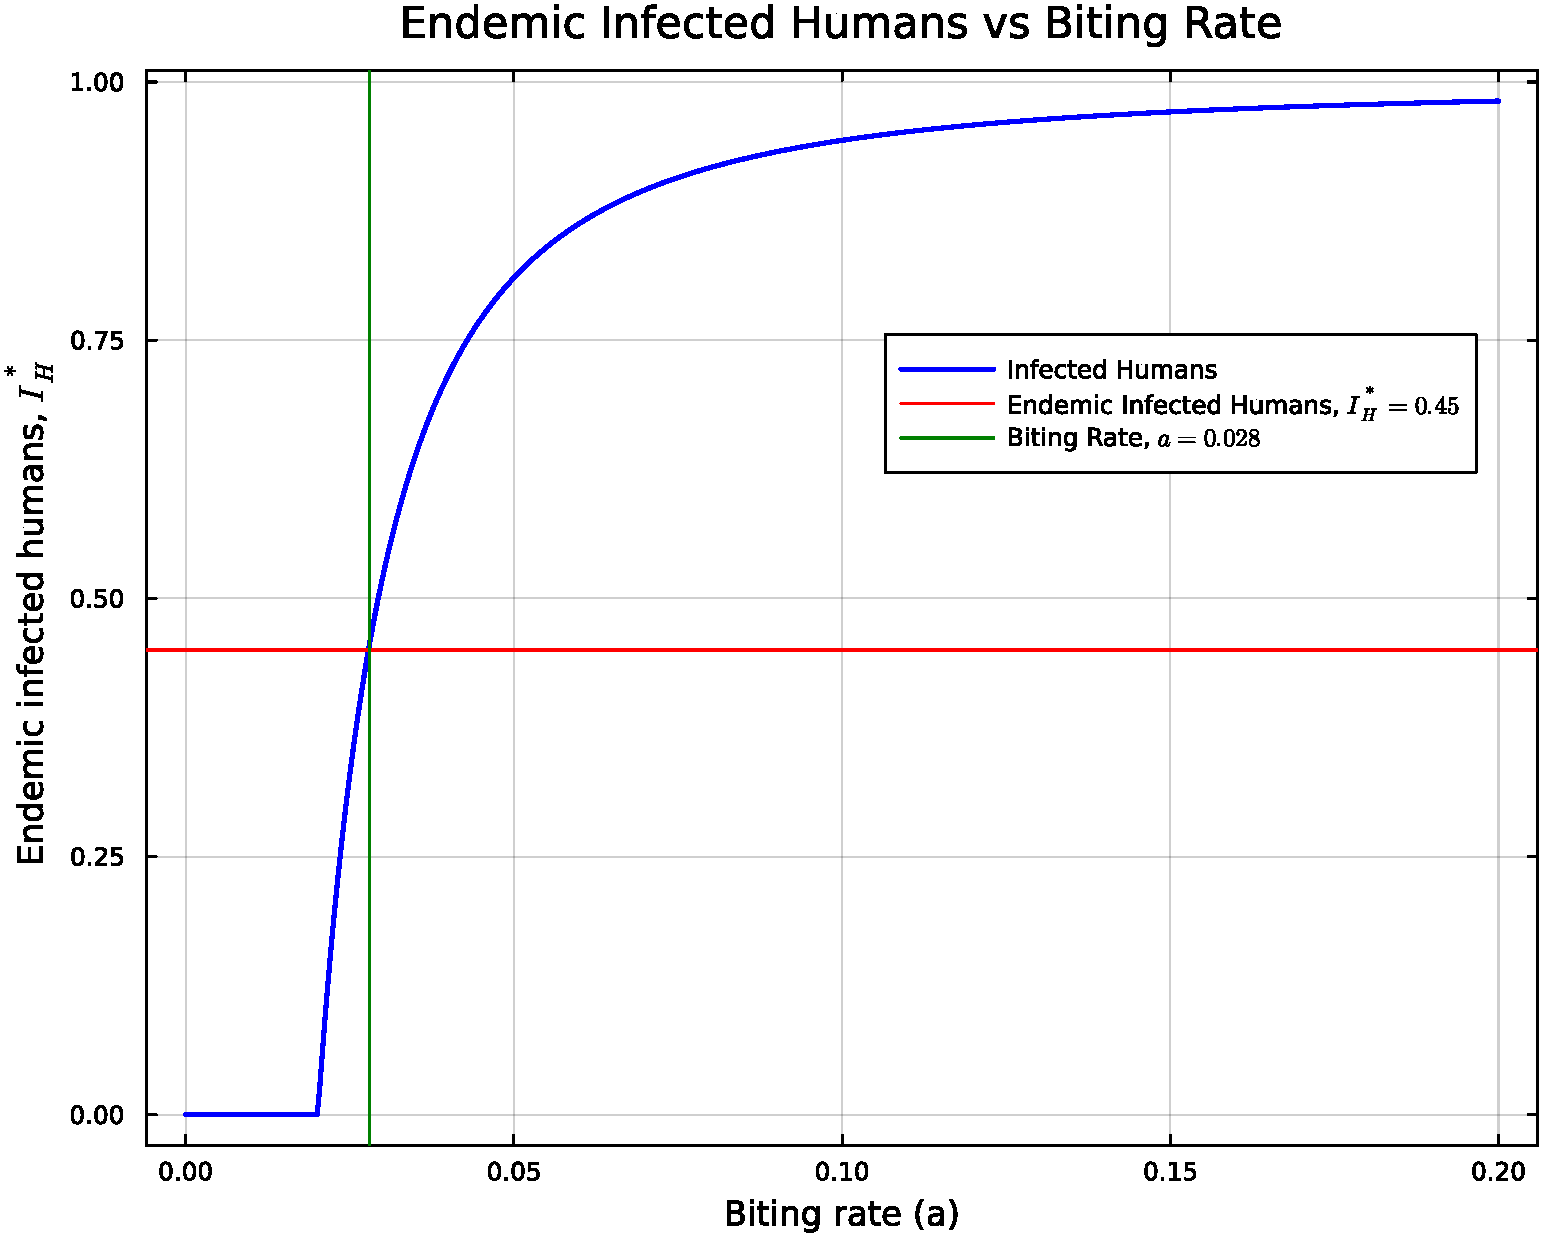
\includegraphics[width=0.8\textwidth]{../../fig/a_cal_PLT.pdf}
  \caption{The plot shows the prevalence of malaria in humans as a function of the biting rate $a$. The red dashed line indicates the target prevalence of 45\%. The blue line shows the prevalence calculated from the model, and the green line shows the required biting rate. Therefore, the biting rate $a$ is calibrated to approximately 0.028 to achieve the target prevalence of 45\%.}
\end{figure}

From now on, we will use the calibrated biting rate $a=0.028$ for all further simulations and analyses. The heatmaps of the basic reproduction number $R_0$ and the human infected proportion $I_H^*$ at equilibrium will be recalculated with this new value of $a$ and are as follows:

\begin{figure}[H]
  \centering
  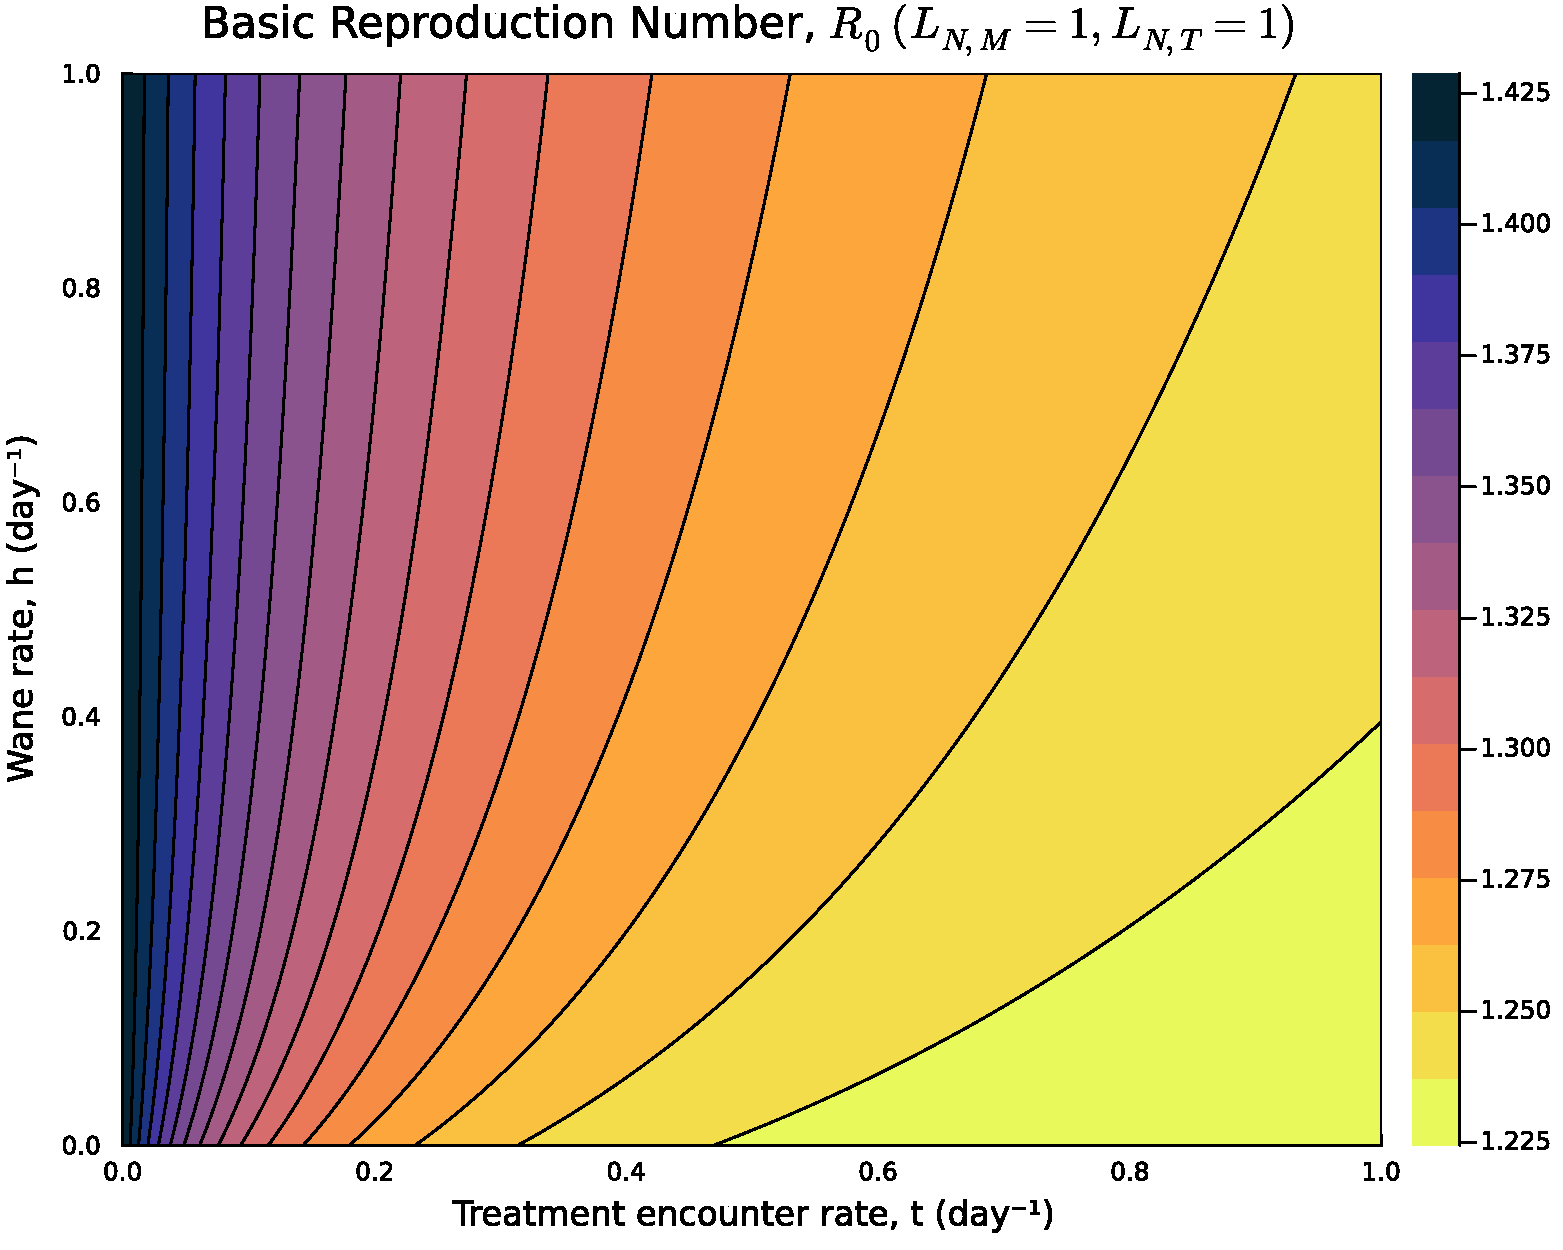
\includegraphics[width=0.4\textwidth]{../../fig/R0_rates_txh_1x1_cal.pdf}
  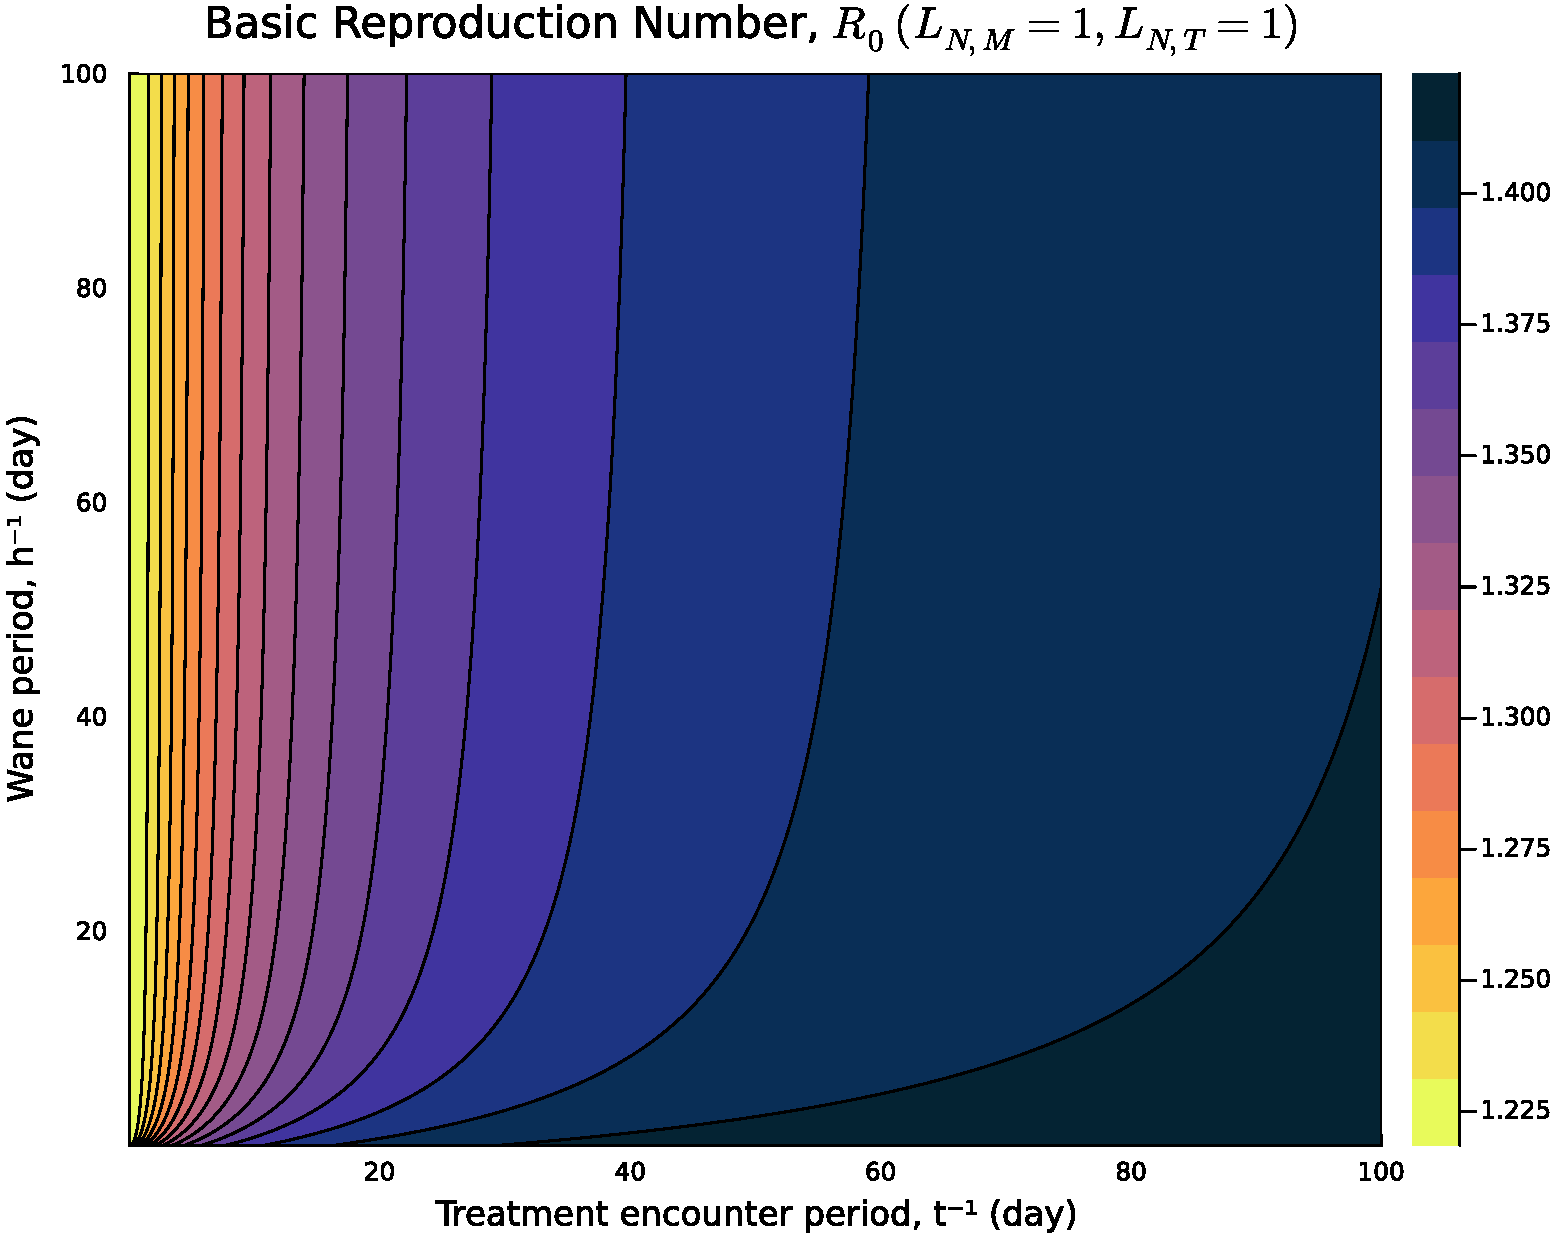
\includegraphics[width=0.4\textwidth]{../../fig/R0_periods_txh_1x1_cal.pdf}\\
  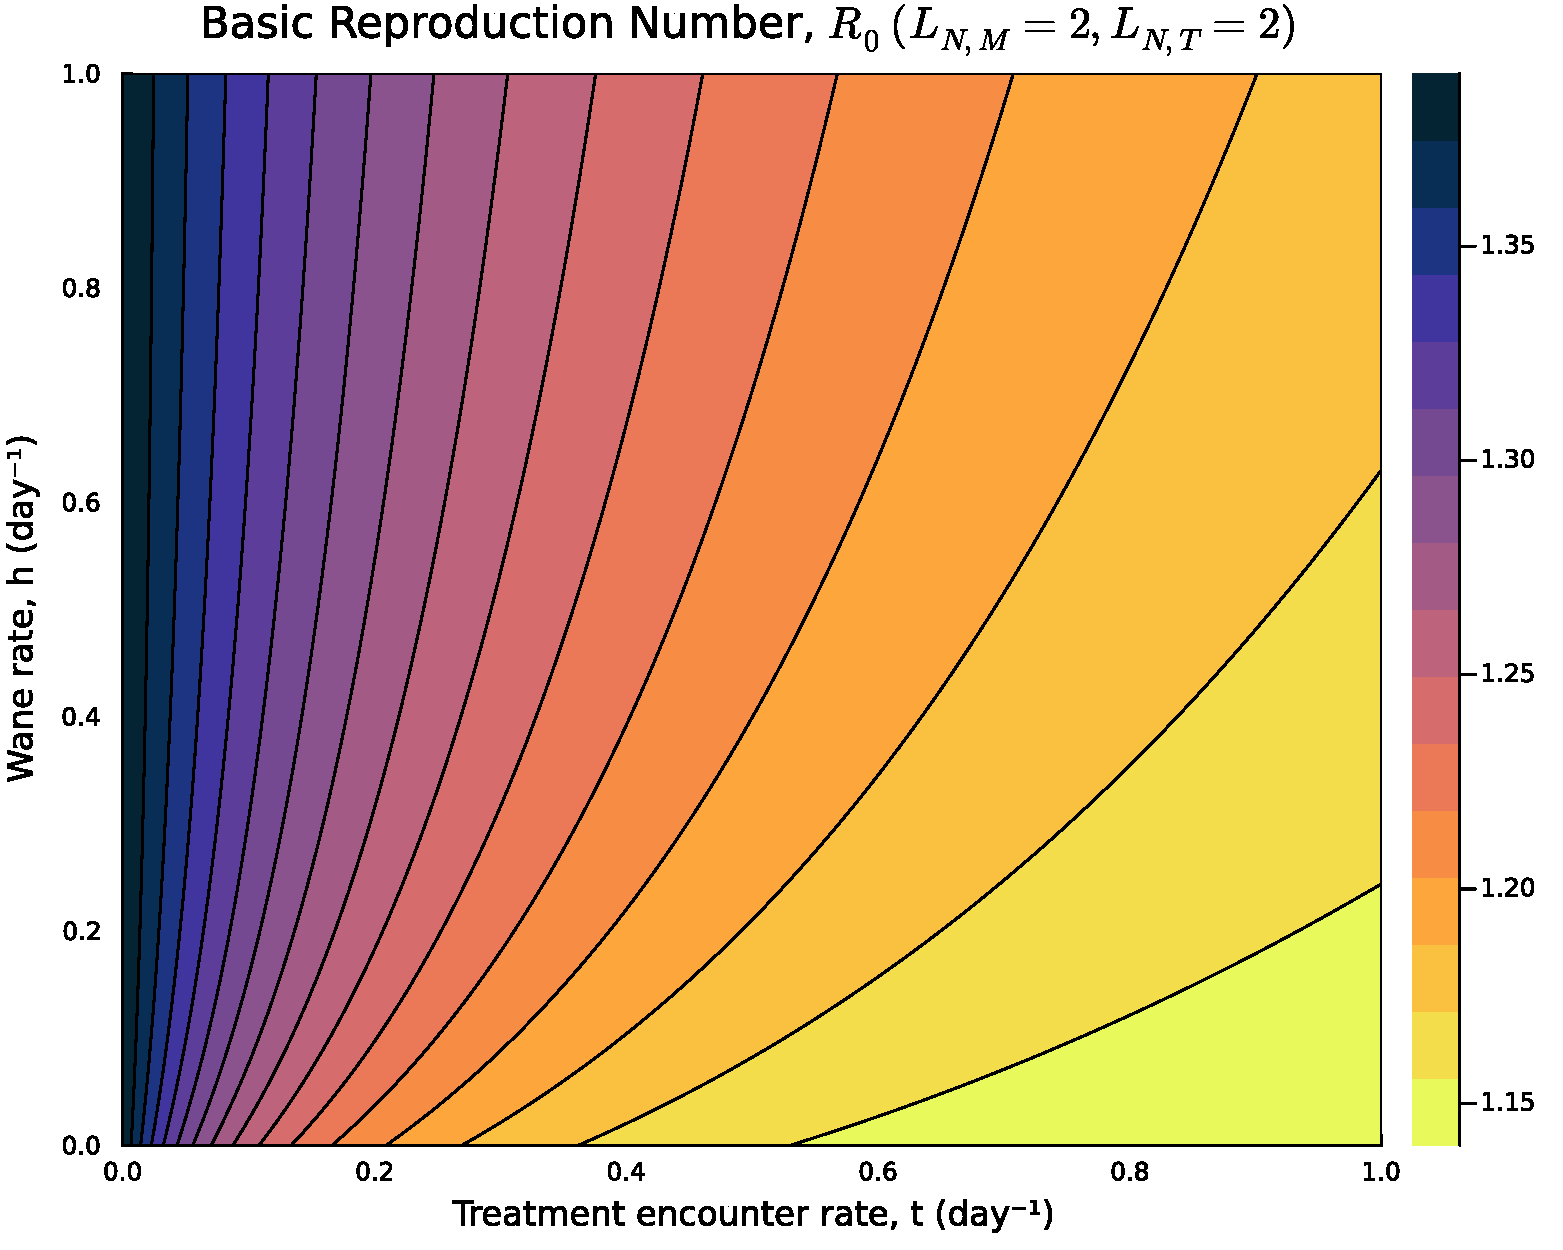
\includegraphics[width=0.4\textwidth]{../../fig/R0_rates_txh_2x2_cal.pdf}
  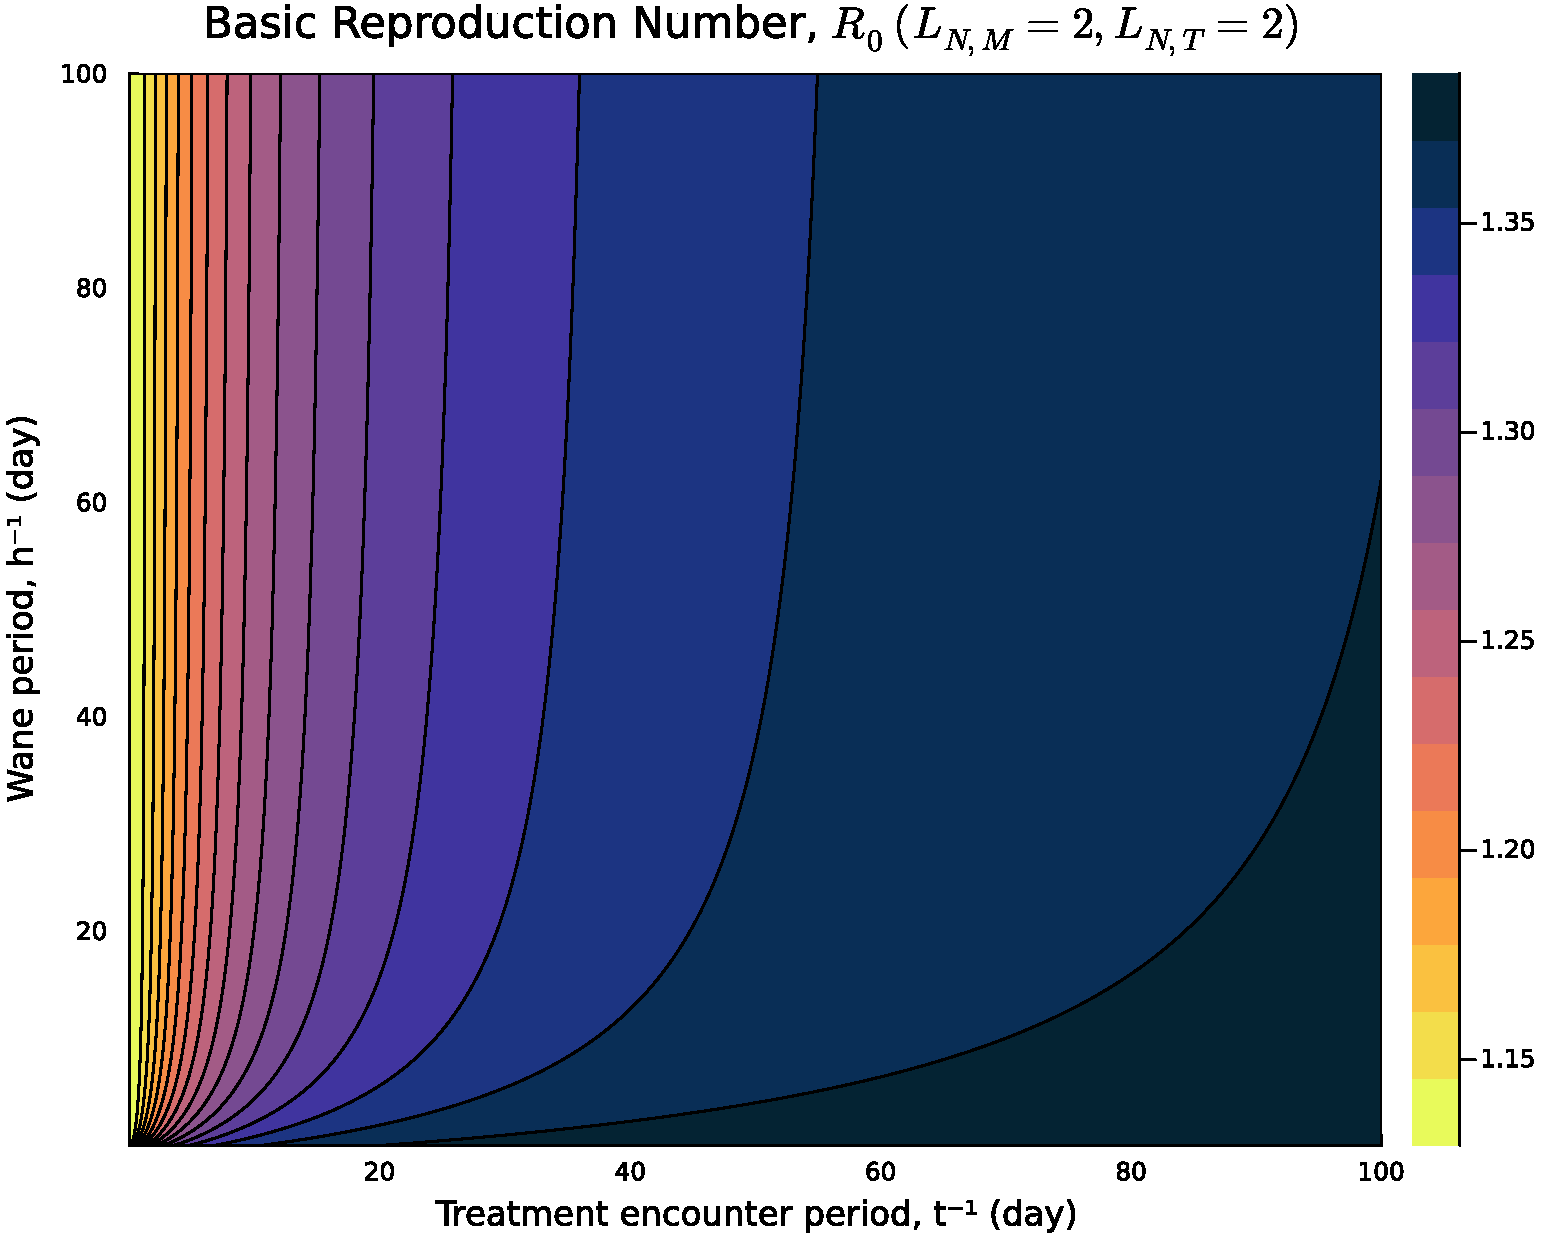
\includegraphics[width=0.4\textwidth]{../../fig/R0_periods_txh_2x2_cal.pdf}\\
  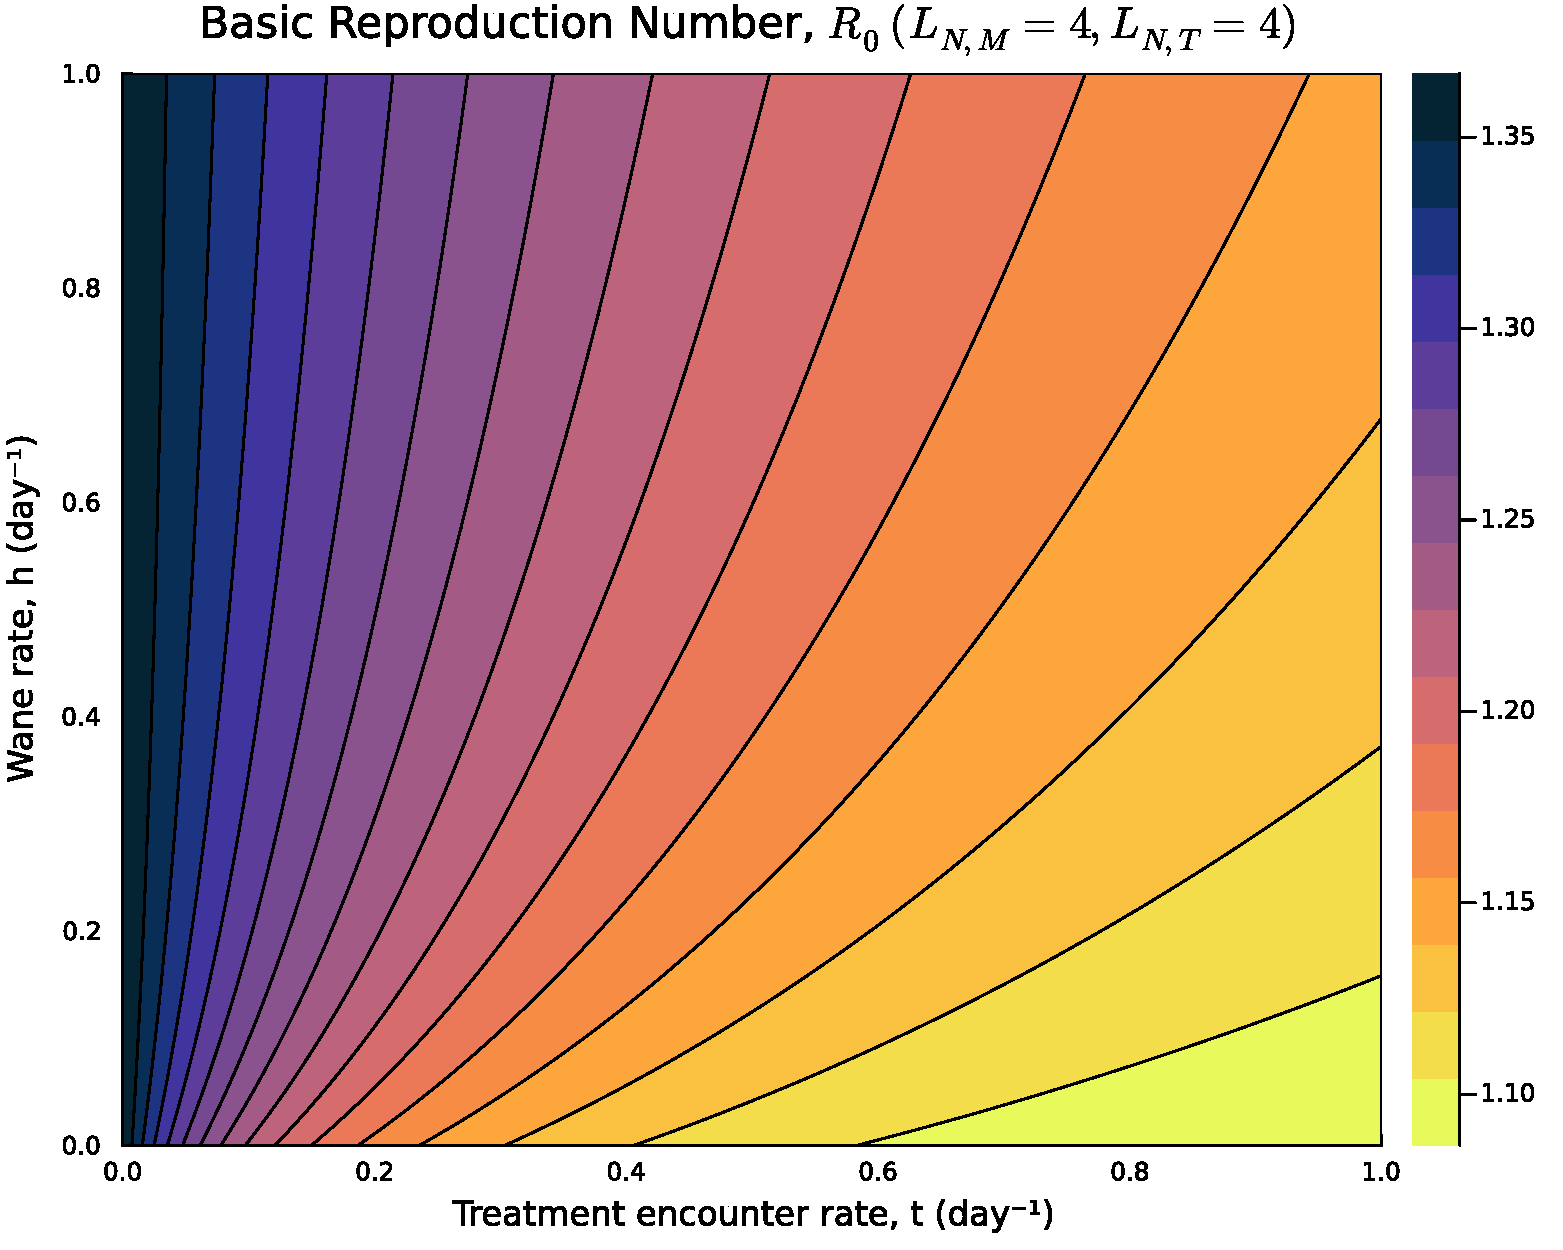
\includegraphics[width=0.4\textwidth]{../../fig/R0_rates_txh_4x4_cal.pdf}
  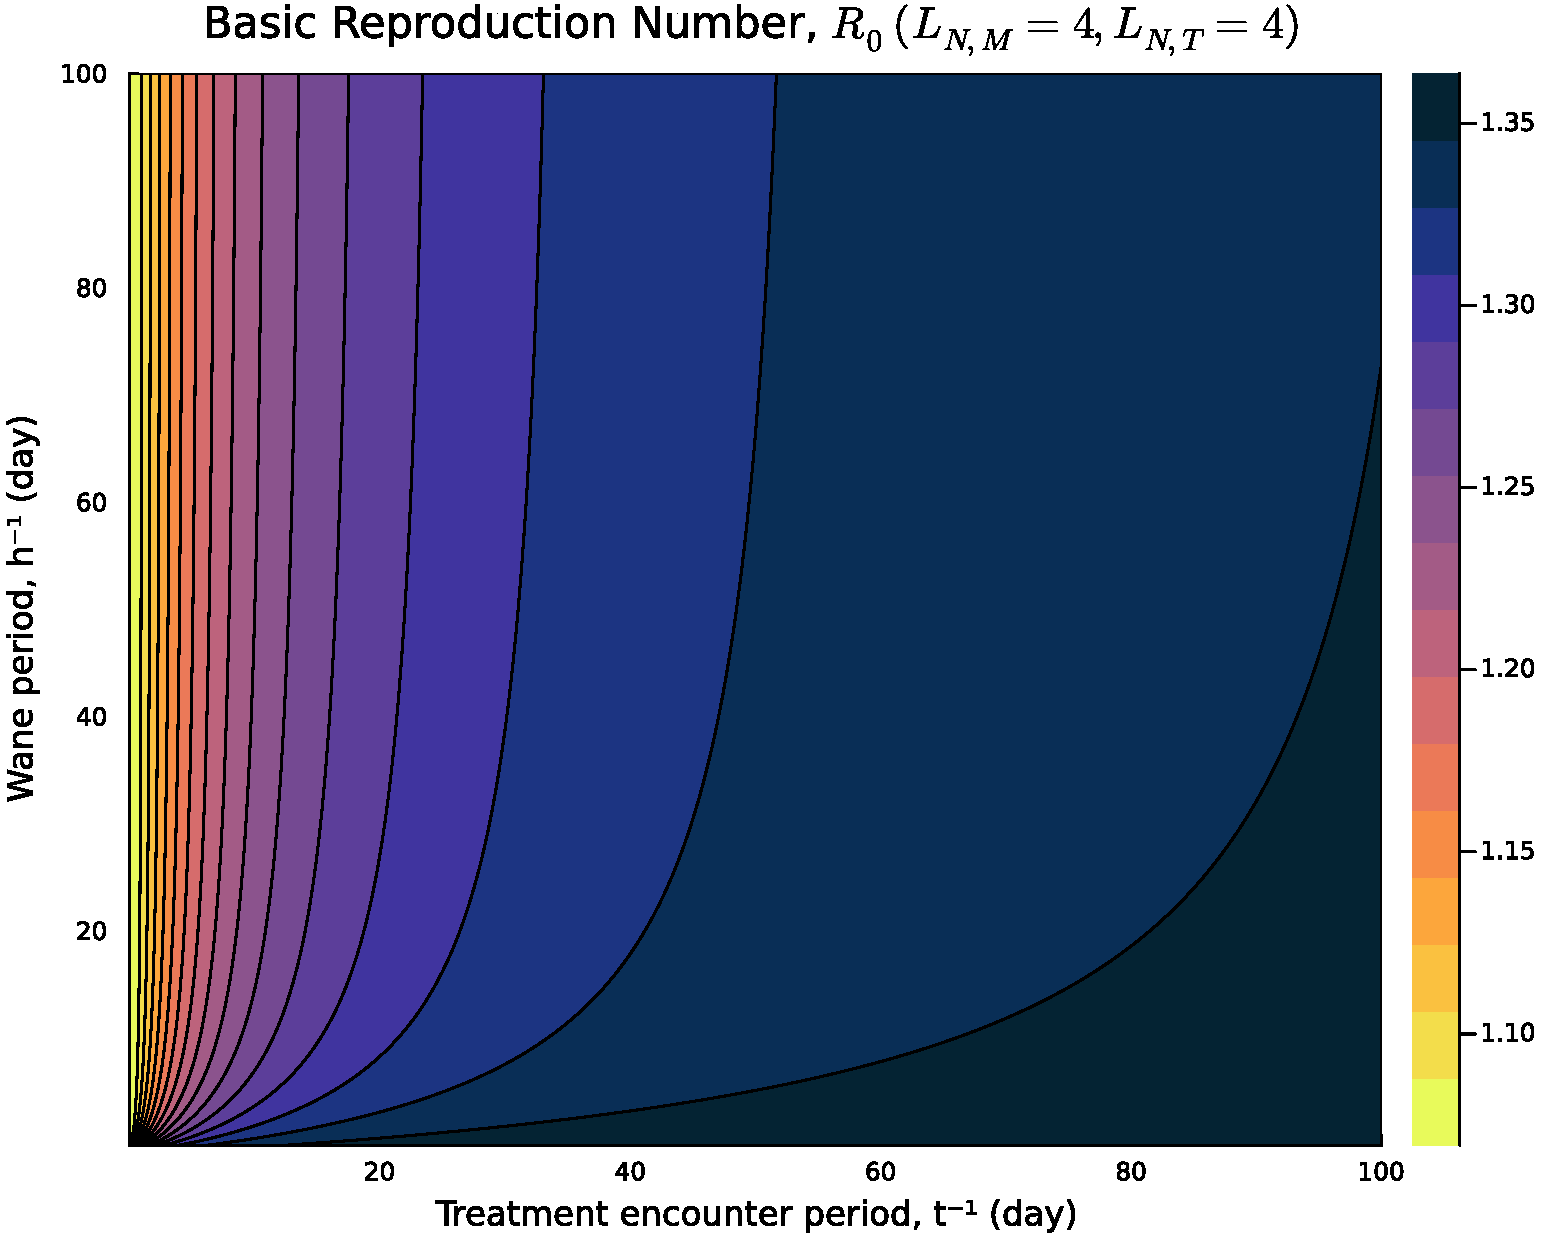
\includegraphics[width=0.4\textwidth]{../../fig/R0_periods_txh_4x4_cal.pdf}
  \caption{Heatmaps of the basic reproduction number $R_0$ as a function of treatment rate $t$ and treatment waning rate $h$ or treatment encounter period $t$ and treatment waning period $h$ for the generalized model with erlang-distributed mosquito latency with 1, 2, and 4 latency stages for both untreated and treated mosquitoes with calibrated biting rate $a=0.028$.}
\end{figure}

\begin{figure}[H]
  \centering
  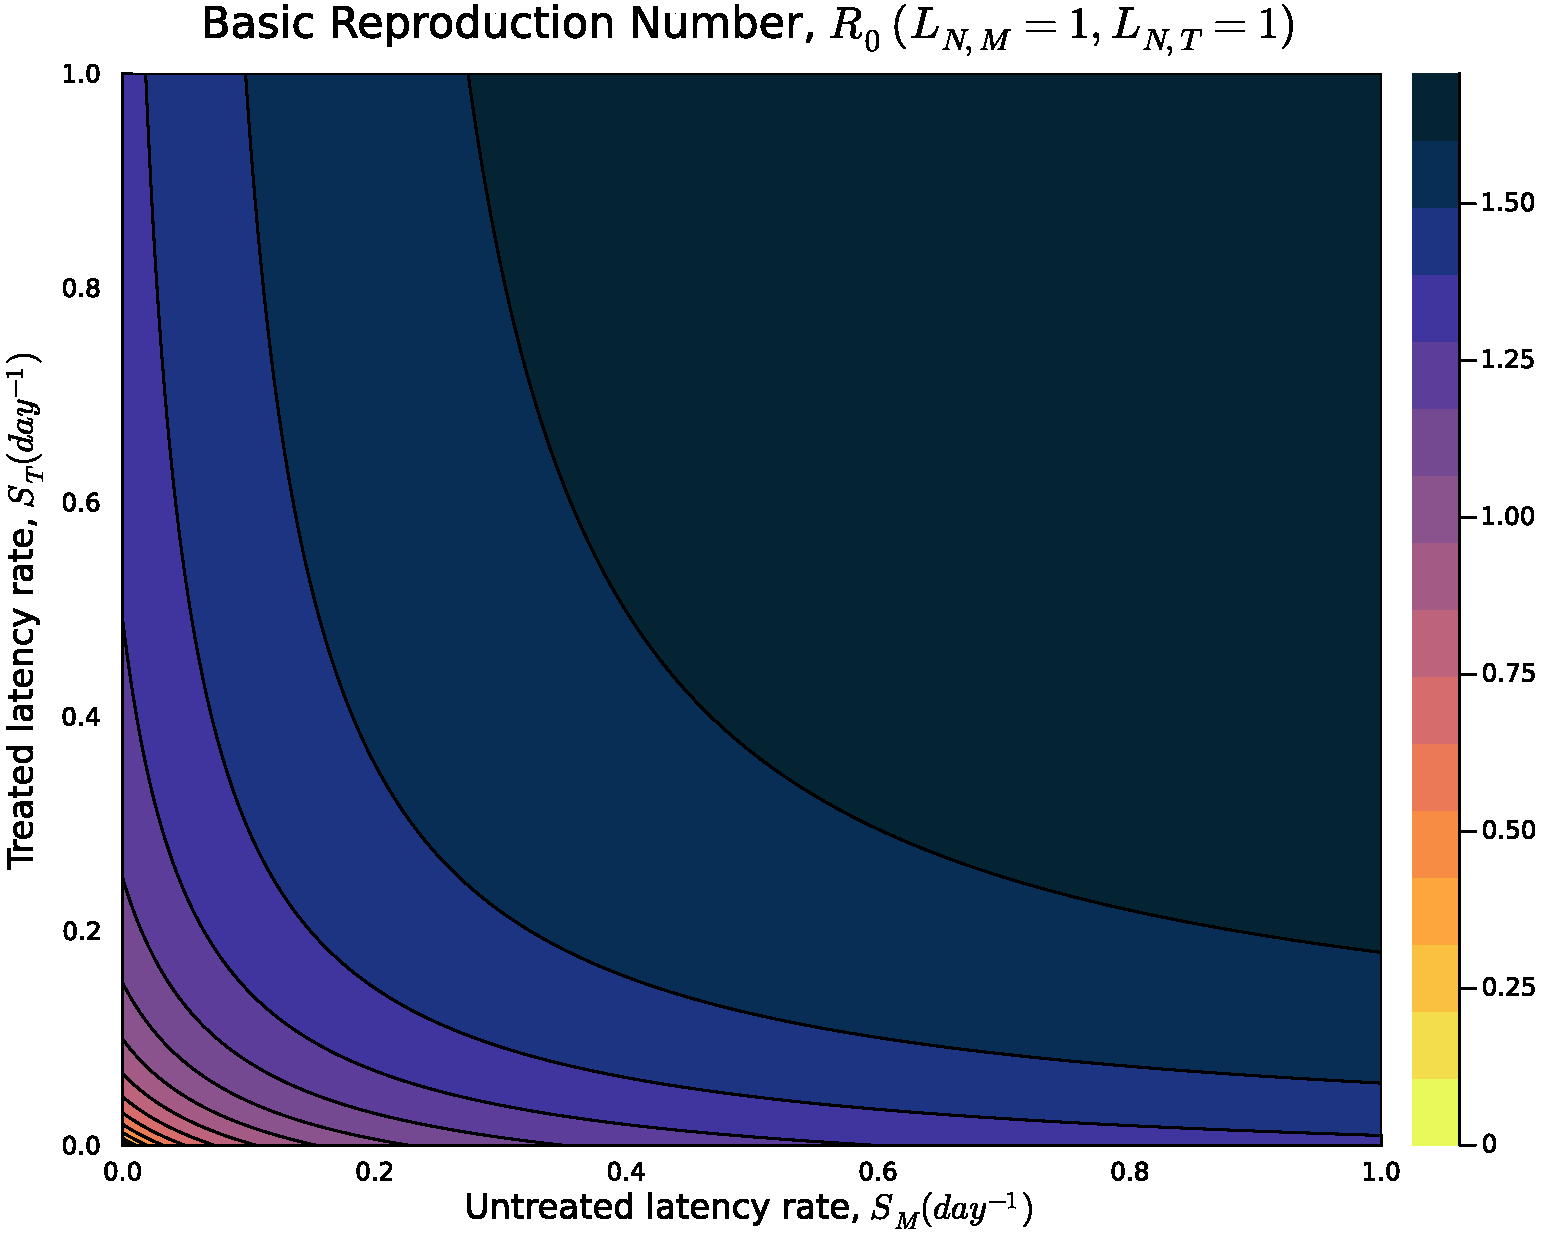
\includegraphics[width=0.4\textwidth]{../../fig/R0_rates_SMxST_1x1_cal.pdf}
  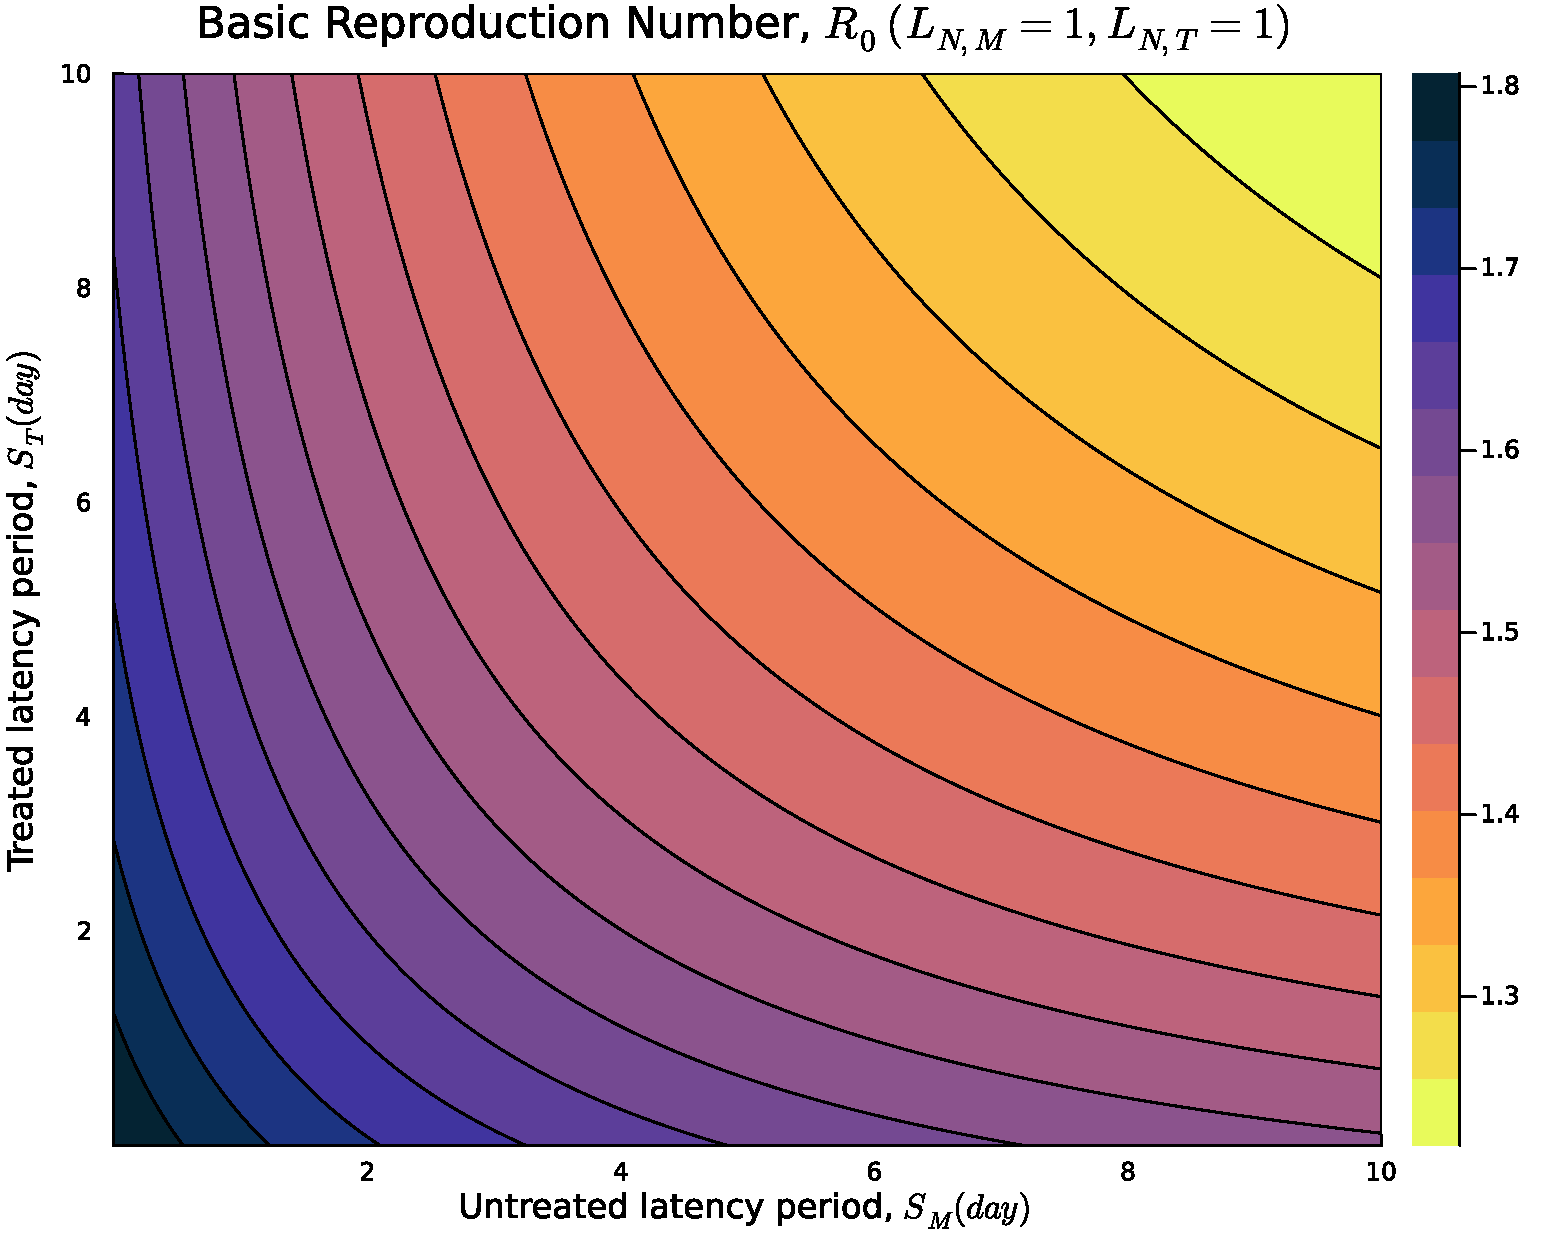
\includegraphics[width=0.4\textwidth]{../../fig/R0_periods_SMxST_1x1_cal.pdf}\\
  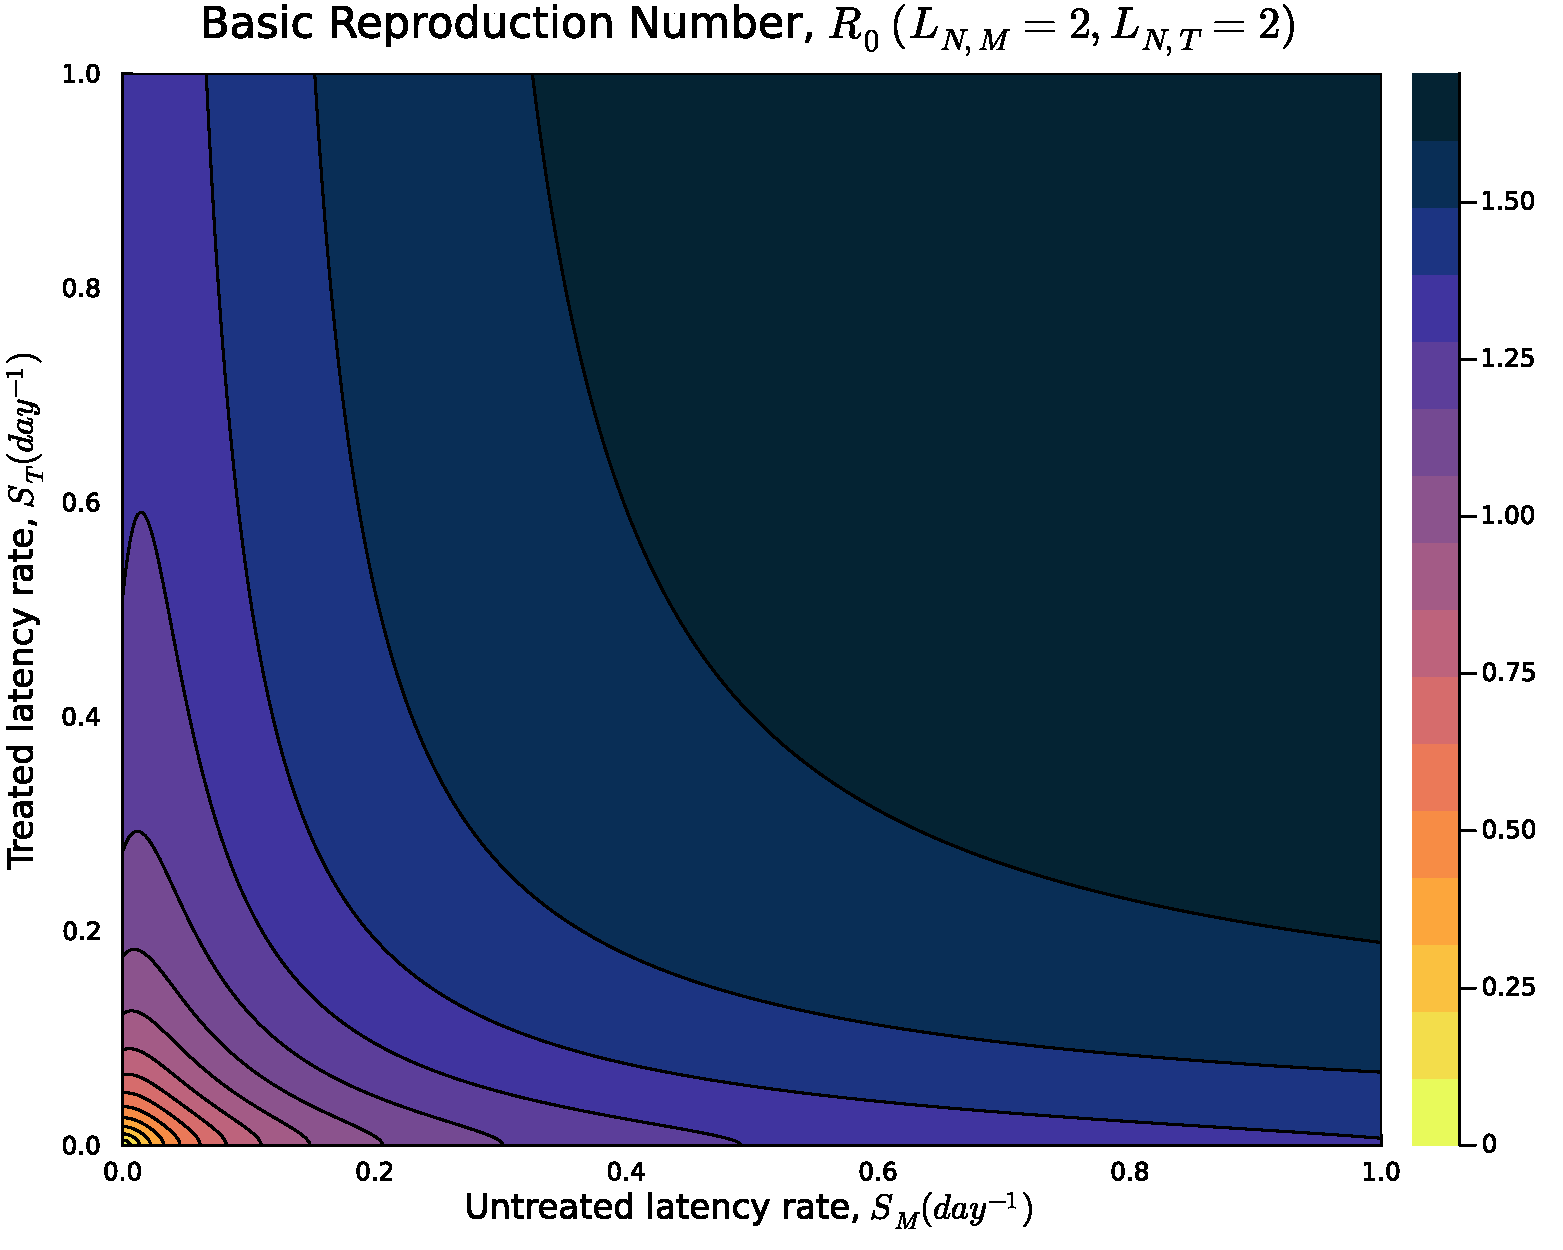
\includegraphics[width=0.4\textwidth]{../../fig/R0_rates_SMxST_2x2_cal.pdf}
  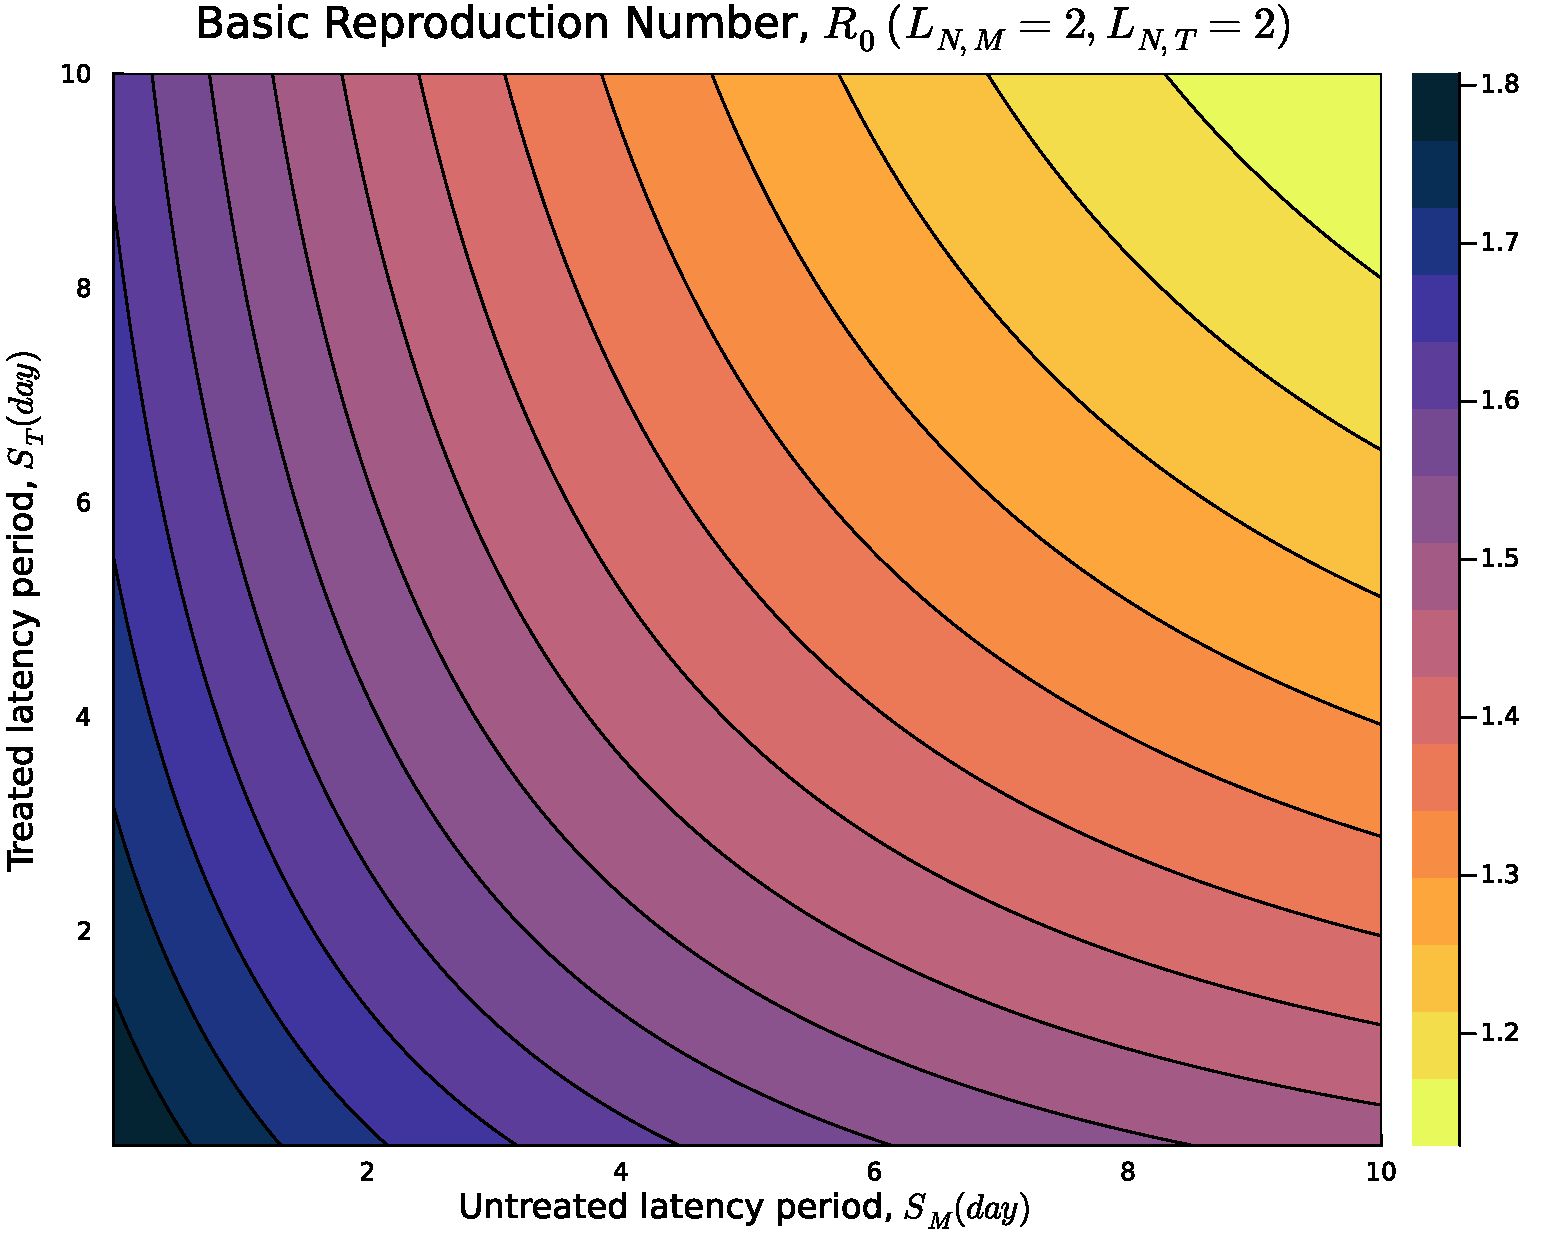
\includegraphics[width=0.4\textwidth]{../../fig/R0_periods_SMxST_2x2_cal.pdf}\\
  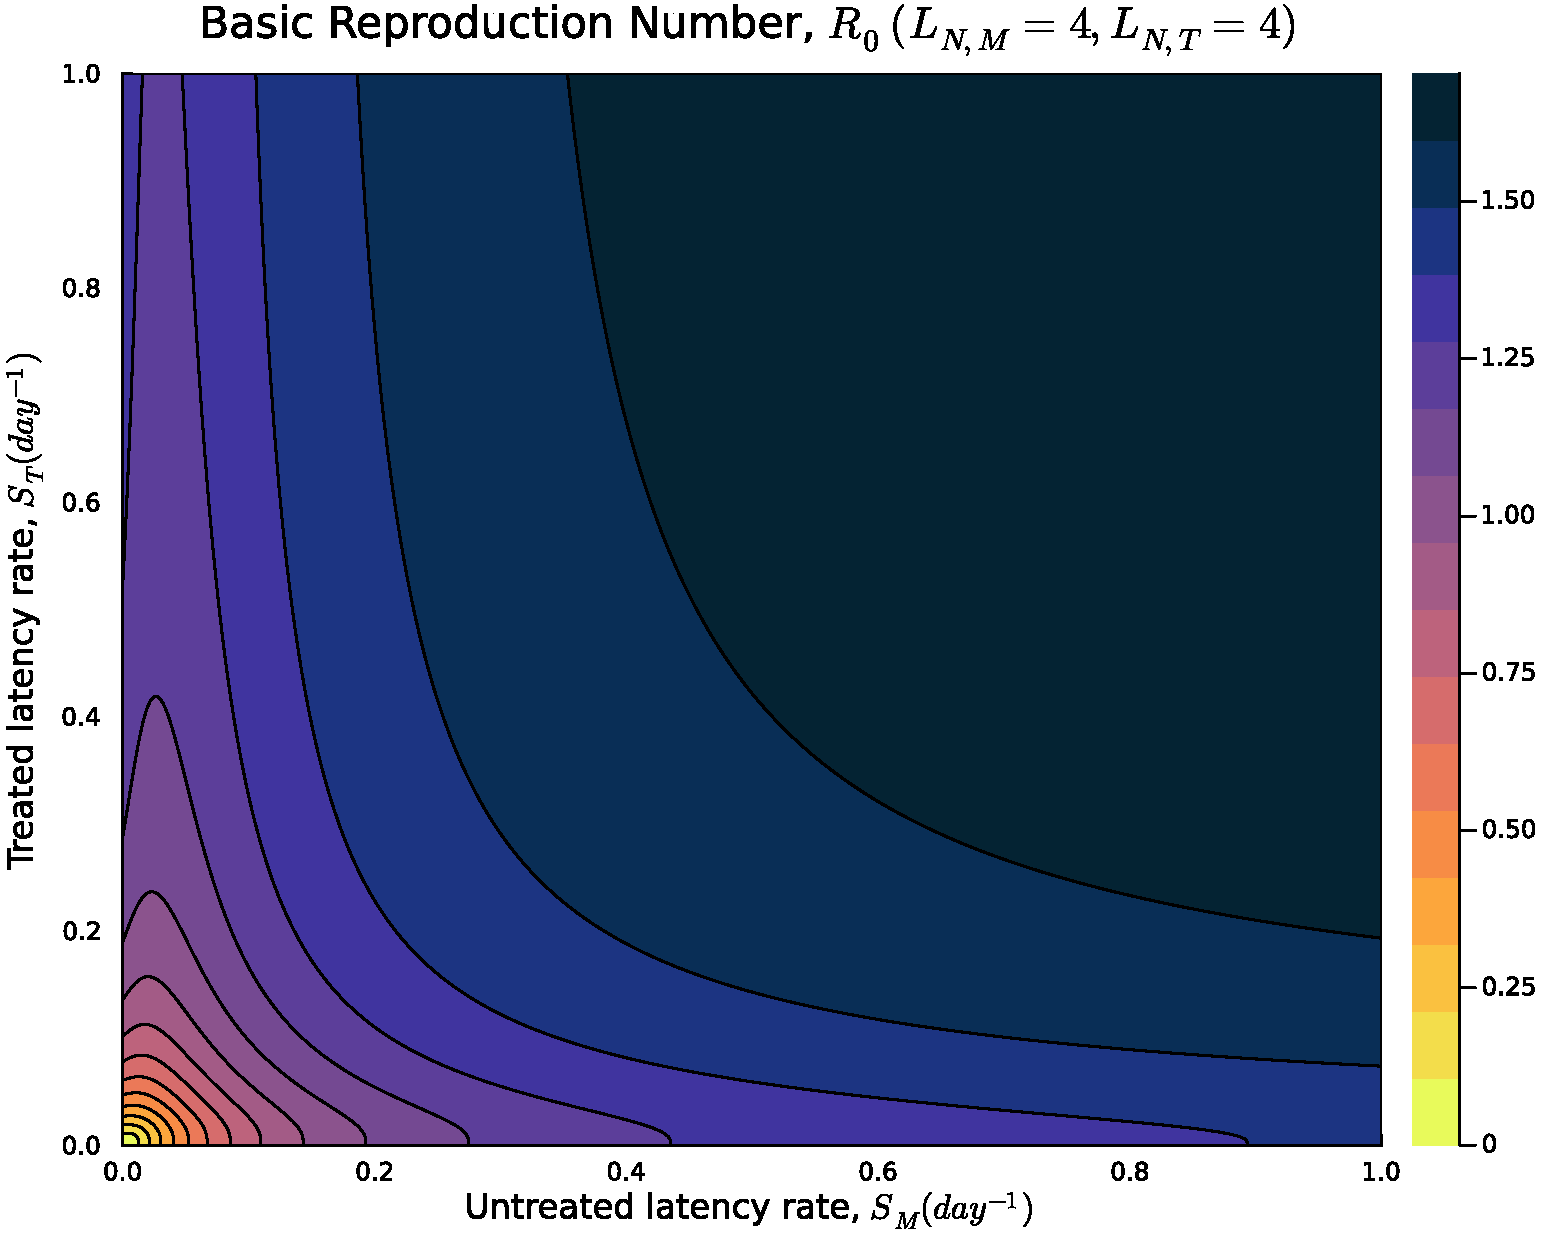
\includegraphics[width=0.4\textwidth]{../../fig/R0_rates_SMxST_4x4_cal.pdf}
  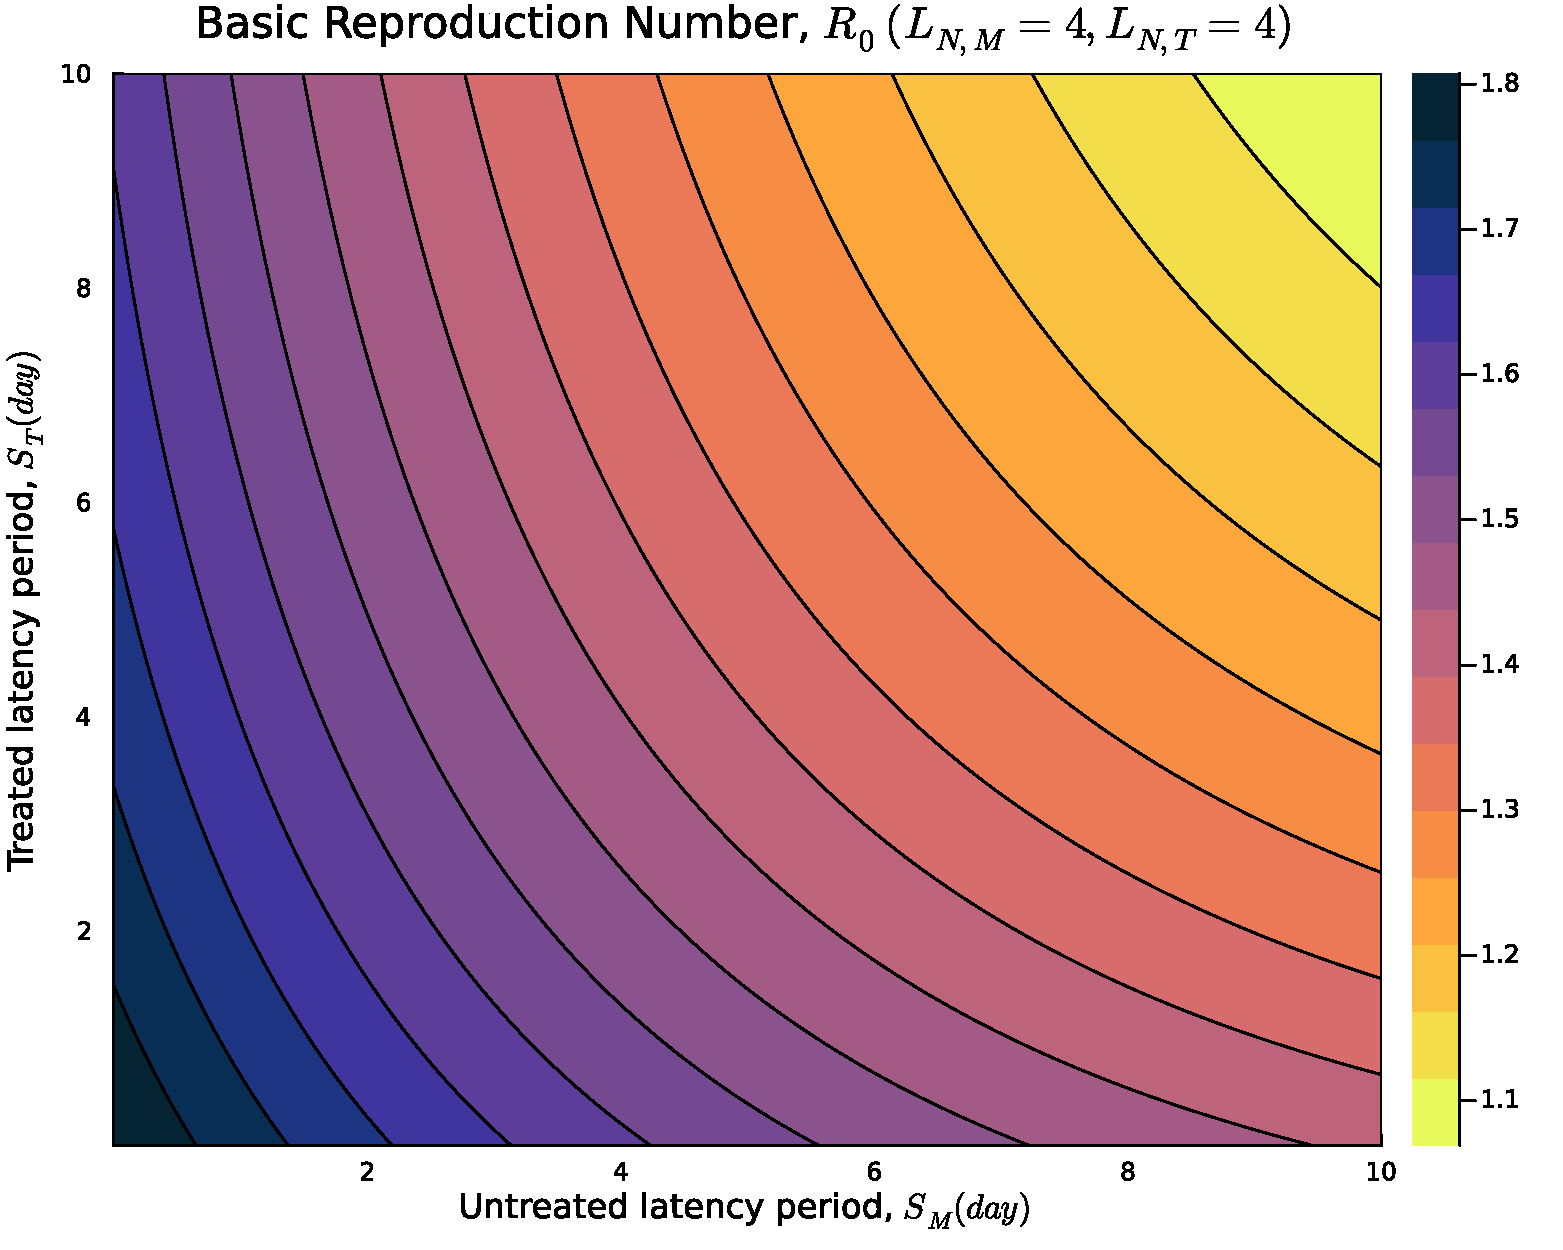
\includegraphics[width=0.4\textwidth]{../../fig/R0_periods_SMxST_4x4_cal.pdf}
  \caption{Heatmaps of the basic reproduction number $R_0$ as a function of untreated mosquito latency progression rate $s_M$ and treated mosquito latency progression rate $s_T$ or untreated mosquito latency period $L_{NM}$ and treated mosquito latency period $L_{NT}$ for the generalized model with erlang-distributed mosquito latency with 1, 2, and 4 latency stages for both untreated and treated mosquitoes with calibrated biting rate $a=0.028$.}
\end{figure}

\begin{figure}[H]
  \centering
  \includegraphics[width=0.4\textwidth]{../../fig/Ih_rates_txh_1x1_cal.pdf}
  \includegraphics[width=0.4\textwidth]{../../fig/Ih_periods_txh_1x1_cal.pdf}\\
  \includegraphics[width=0.4\textwidth]{../../fig/Ih_rates_txh_2x2_cal.pdf}
  \includegraphics[width=0.4\textwidth]{../../fig/Ih_periods_txh_2x2_cal.pdf}\\
  \includegraphics[width=0.4\textwidth]{../../fig/Ih_rates_txh_4x4_cal.pdf}
  \includegraphics[width=0.4\textwidth]{../../fig/Ih_periods_txh_4x4_cal.pdf}
  \caption{Heatmaps of the human infected proportion $I_H^*$ at equilibrium (prevalence) as a function of treatment rate $t$ and treatment waning rate $h$ or treatment encounter period $t$ and treatment waning period $h$ for the generalized model with erlang-distributed mosquito latency with 1, 2, and 4 latency stages for both untreated and treated mosquitoes with calibrated biting rate $a=0.028$.}
\end{figure}

\begin{figure}[H]
  \centering
  \includegraphics[width=0.4\textwidth]{../../fig/Ih_rates_SMxST_1x1_cal.pdf}
  \includegraphics[width=0.4\textwidth]{../../fig/Ih_periods_SMxST_1x1_cal.pdf}\\
  \includegraphics[width=0.4\textwidth]{../../fig/Ih_rates_SMxST_4x4_cal.pdf}
  \includegraphics[width=0.4\textwidth]{../../fig/Ih_periods_SMxST_4x4_cal.pdf}
  \caption{Heatmaps of the human infected proportion $I_H^*$ at equilibrium (prevalence) as a function of untreated mosquito latency progression rate $s_M$ and treated mosquito latency progression rate $s_T$ or untreated mosquito latency period $L_{NM}$ and treated mosquito latency period $L_{NT}$ for the generalized model with erlang-distributed mosquito latency with 1, 2, and 4 latency stages for both untreated and treated mosquitoes with calibrated biting rate $a=0.028$.}
\end{figure}

\end{document}
